% !TEX TS-program = pdflatex
% !TEX encoding = UTF-8 Unicode

% This is a simple template for a LaTeX document using the "article" class.
% See "book", "report", "letter" for other types of document.

\documentclass[11pt]{article} % use larger type; default would be 10pt

\usepackage[utf8]{inputenc} % set input encoding (not needed with XeLaTeX)
\usepackage{hyperref}
\usepackage{graphics}
\usepackage{mathrsfs}
\usepackage{rotating}


%%% Examples of Article customizations
% These packages are optional, depending whether you want the features they provide.
% See the LaTeX Companion or other references for full information.

%%% PAGE DIMENSIONS
\usepackage{geometry} % to change the page dimensions
\geometry{a4paper} % or letterpaper (US) or a5paper or....
% \geometry{margin=2in} % for example, change the margins to 2 inches all round
% \geometry{landscape} % set up the page for landscape
%   read geometry.pdf for detailed page layout information

\usepackage{graphicx} % support the \includegraphics command and options

% \usepackage[parfill]{parskip} % Activate to begin paragraphs with an empty line rather than an indent

%%% PACKAGES
\usepackage{booktabs} % for much better looking tables
\usepackage{array} % for better arrays (eg matrices) in maths
\usepackage{paralist} % very flexible & customisable lists (eg. enumerate/itemize, etc.)
\usepackage{verbatim} % adds environment for commenting out blocks of text & for better verbatim
\usepackage{subfig} % make it possible to include more than one captioned figure/table in a single float
% These packages are all incorporated in the memoir class to one degree or another...

%mike
\usepackage[authoryear]{natbib}
\usepackage{fullpage}
\usepackage{setspace}
\onehalfspacing
% added by mike to get "th"'s and "`sts"' working
\usepackage{xspace}
\newcommand\nd{\textsuperscript{nd}\xspace}
\newcommand\rd{\textsuperscript{rd}\xspace}
\newcommand\nth{\textsuperscript{th}\xspace} 

% added by mike to get author's and affiliations http://tex.stackexchange.com/questions/9594/adding-more-than-one-author-with-different-affiliation
\usepackage{authblk}

% added by mike to automatically convert eps to pdf. pdflatex cant cope with eps files.
% http://tex.stackexchange.com/questions/69355/why-doesnt-latex-allow-me-to-import-my-eps-file-when-i-compile-it
\usepackage{epstopdf}

%%% HEADERS & FOOTERS
\usepackage{fancyhdr} % This should be set AFTER setting up the page geometry
\pagestyle{fancy} % options: empty , plain , fancy
\renewcommand{\headrulewidth}{0pt} % customise the layout...
\lhead{}\chead{}\rhead{}
\lfoot{}\cfoot{\thepage}\rfoot{}

%%% SECTION TITLE APPEARANCE
\usepackage{sectsty}
\allsectionsfont{\sffamily\mdseries\upshape} % (See the fntguide.pdf for font help)
% (This matches ConTeXt defaults)

%%% ToC (table of contents) APPEARANCE
\usepackage[nottoc,notlof,notlot]{tocbibind} % Put the bibliography in the ToC
\usepackage[titles,subfigure]{tocloft} % Alter the style of the Table of Contents
\renewcommand{\cftsecfont}{\rmfamily\mdseries\upshape}
\renewcommand{\cftsecpagefont}{\rmfamily\mdseries\upshape} % No bold!

%%% END Article customizations

%%% The "real" document content comes below...

\title{Who are the poorest in the UK? Measuring poverty with income and consumption}
\author[1]{Abi Adams}
\author[2]{Mike Brewer}
\author[3]{Cormac O'Dea\thanks{Correspondence to mbrewer@essex.ac.uk. We are very grateful to Thomas Crossley, Ben Etheridge, Robert Joyce, Laura Keyse, Richard Tonkin and Karen Watkins for useful conversations, and to seminar participants at the IFS, the University of Essex, the University of Sheffield, and [mike check name] the 2013 EUROMOD research workshop. The authors gratefully acknowledge funding from the ESRC Centre for the Microeconomic Analysis of Public Policy (Adams and O'Dea) and from the ESRC Research Centre on Micro-social Change (Brewer). The Living Cost and Food Survey and its predecessors, and the Family Resources Survey, are Crown copyright and are reproduced with the permission of the Controller of HMSO and the Queen's Printer for Scotland, and are available from the UK Data Service. The UKDS, the original owners of the data (the Office for National Statistics) and the copyright holders bear no responsibility for their further analysis or interpretation. An earlier version of this paper was circulated under the title ``Measuring living standards with income and consumption: evidence from the UK''.}
}
\affil[1]{Yale University and Institute for Fiscal Studies}
\affil[2]{University of Essex and Institute for Fiscal Studies}
\affil[3]{Institute for Fiscal Studies}
\renewcommand\Authands{ and }

%\date{} % Activate to display a given date or no date (if empty),
         % otherwise the current date is printed 

\begin{document}

\maketitle

\begin{abstract}
%\vspace{-1.5cm}
%\include{ABOD_abstract}
Analysis of trends in poverty, or of the composition of the poor, require an assessment of the living standards of households. Despite theoretical reasons to prefer the use of consumption over income as a general measure of a household's living standards, and practical reasons to prefer the use of consumption to identify the poorest, in developed countries it is common to use poverty lines defined with respect to household income. With a long span of survey-based micro-data on income and consumption for the same households, we contrast the different impressions one gets when using household income or household consumption to assess the trends in low living standards, and the composition of those in poverty. We find that moving from low income to low consumption as a measure of poverty identifies households that are more likely to have low permanent resources, as does adding the implicit income or consumption from housing, as standard economic theory would suggest. [We also show that adding the implicit income or consumption from housing to a measure of household resources has dramatic impacts on the age- and cohort-profile of poverty in the UK]. \end{abstract}



\section{Introduction} 

Point of this paper: comprehensive review of the trends in inequality, and in the level and composition of poverty that one gets with different measures of household resources. 

Measurements of inequality or poverty require us to measure the living standards achieved by, or the resources available to, households. There is a long debate over whether this is best done with income or consumption. Despite theoretical reasons to prefer the use of consumption as a general measure of a household's living standards (\cite{Poterba1989}, Cutler and Katz (1992), Slesnick (1993)), and practical reasons to prefer the use of consumption to identify the poorest (Meyer and Sullivan 2003, 2004, 2008, 2011; Meyer, Kok (or Bee?and Sullivan); Brewer, Etheridge and O'Dea, forthcoming. [Mike NEEDs to CHECK TO FIND OUT WHICH ARE ABOUT MEASUREMENT ISSUES]), it is common in developed countries to assess inequality with respect to the distribution of household income, and to use poverty lines defined with respect to household income. 

However, these arguments for or against the use of consumption rather than income are of little practical importance if trends in living standards, inequality or poverty were similar for the two measures, and if the set of households with a low consumption were the broadly similar to those with a low income. Using a long span of consistent survey-based micro-data on income and consumption for the same households, this paper therefore assesses what impact the way we measure household resources has on our impression of trends in the level and distribution of living standards, and the composition of those in poverty in the UK. 

In doing this, we develop the findings of Brewer, Etheridge and O'Dea (forthcoming), which documents thoroughly the mis-match between reported income and reported spending for households with low resources in the UK and presents evidence that this is much more likely to be due to under-reporting of income than either over-reporting of spending or consumption-smoothing. We stress, though, that even if one takes a different view on the underlying causes, the significant mismatch between measures of income and consumption for households with low resources remains, and it is important to know to what extent income and consumption give different impressions of trends in, and the composition of, households with low resources. 

Our broad approach is to analyse (and then compare) the trends in the level and distribution of households' resources, and the risk factors of having low resources, using both income and consumption as our measure of household resources. In doing so, we pay particular attention to the role of the implicit rental income derived from, or the implicit consumption flow from, owner-occupied housing.

We go beyond the literature in three main ways - first long time span

explicit consideration of the role of implicit rental income/consumption of housing 

This is important for two reasons. First, some work which has compared the use of income and consumption to measure well-being has, in effect, compared a measure of disposable, cash, incomes with a measure of full consumption, including the consumption flows from durables, such as housing ([justify this!]). This is an unfair comparison; it is just as sensible to think that consumer durables provide their owners with an implicit stream of rental income as it is to think that they provide an implicit stream of consumption (and we must think in this way if we work with the Haig-Simons concept that income less consumption equals change in net worth). Instead, we proceed by first comparing the usual measure of disposable cash income with an equivalent measure of consumption, and then assessing what changes when we add to these the implicit rent or consumption flow from housing.  Second, despite the recommendations of the Canberra Group on measuring income ([reference]), all official and most academic analysis of household incomes in the UK uses an income concept that does not include implicit rental income (and the partial availability of data on implicit rental income means that most international comparisons do likewise; see, e.g., Morelli et al (2015) [handbook chapter]), and our analysis therefore presents the most comprehensive assessment of what impact including the implicit rent from home ownership [Mike says: we must agree and then standardise how I refer to this; I used a different phrase in chapters 4-6] would have on an analysis of the income distribution in the UK.    

Our results can be grouped into four areas. 

First, we find that the distribution of income and consumption are quite different, in every year of our data. There was little difference between summary measures of inequality in income and consumption in the first half of the 1980s, but income inequality then grew considerably faster, where it remains less equally distributed than consumption. [Or: ``Inequality and relative poverty grew less rapidly when measured with consumption, partly because consumption at the bottom grew more strongly than income in the 1980s, and because consumption at the top grew less strongly than income in the 1990 and 2000s [Mike notes: text following "`partly"' not all shown in this paper.]'']. A similar story is true for measures of relative poverty (having a household income, or consumption, below 60\% of the national median). [Resources have grown by more when assessed using income than consumption (particularly in the late 1980s and late 2000s).]  

Second, we present empirical evidence that the set of households with a low consumption are more likely to reflect households who have low permanent resources, as standard economic theory would suggest, than the set of households with a low income. Although this does not necessarily mean that policy-makers should target anti-poverty programmes on those with a low consumption, it does mean that one should look at consumption as well as/instead of income when assessing trends in poverty, and particularly when assessing which groups in society are at risk of poverty. [Mike asks Abi and Cormac: having written this, I feel like resurrecting the DiD analysis that Cormac did, directly assessing how well consumption and income are at identifying the deprived!]. 

Third, at an aggregate level, we show that adding the implicit income or consumption from housing to measures of household resources makes a substantial difference to average annual growth rates in household living standards over the past 30 years, even after an appropriate correction to the price deflator [, and particular so for elderly households] [Mike notes: last bit was in Brewer and O'Dea but is not currently shown in this paper], and also reduces the apparent growth in inequality in household resources. 

Fourth, at a micro-level, moving to a measure of resources that includes 
the implicit income or consumption from housing alters the characteristics of those deemed to be poor by giving less weight [wrong phrase] to those more likely to be temporarily poor (the unemployed and those with high education);



The rest of the paper is arranged as follows.  Section \ref{sec:literature} provides a literature review. Section \ref{sec:measure} discusses how we construct measures of consumption and income from 30 years worth of household surveys.  Section \ref{sec:trends} compares how living standards in the UK have changed over the past 30 years when assessed with household income and household consumption, and examines trends in summary measures of inequality and poverty. Section \ref{sec:composition} examines how our impression of who is poor changes when we switch from using income to using consumption as the measure of resources. Section \ref{sec:housing} assesses how important is the treatment of implicit income from housing when constructing measures of household living standards. Section \ref{sec:conclusion} concludes. Appendices provide more detail on the underlying data sources, and supplementary results.

\section{Related Literature}\label{sec:literature}

%[Mike notes: I have not worked on this recently and there are many papers to add. The idea is to first cite key works on "why use consumption", and then give a more thorough review of papers that directly compare the 2, then cite all the UK stuff, and then the odds and sods at the end.]

Our approach in this paper is not to argue that consumption is a better or worse measure of living standards than income, but to accept that consumption and income are often different measures, even for the same household, and to ask how this changes our impression of how the distribution of household resources in the UK has changed over time, and how it changes the composition of the poor. \footnote{This is complementary to the strand of the literature that studies changes over time in the joint distribution of income and consumption to try to understand the relative importance of temporary and permanent shocks to income; this includes, for example, Krueger and Perri (2006), Attanasio et al (2009) and Blundell et al (2008) which use US data, and Blundell and Preston (1996, 1998), Blundell and Etheridge (2010) and Blundell et al (2013) for the UK.} 

Several papers have asked similar questions for the US, with the most-studied issue being whether inequality in consumption in the US has grown by as much as inequality in income over the past few decades. The general conclusion of the first papers in this literature was that consumption inequality had grown by less than income inequality through the 1980s and 1990s (see, for example, Krueger and Perri (2006) and citations within, Heathcote et al. (2010), Meyer and Sullivan (2013) [5 decades]), although more recently more papers (e.g. Fisher et al. (2014), Aguiar and Bils (2015) and Attanasio et al. (2015)) have concluded that over a long period of time, the rise in inequality looks similar assessed on either measure (and this despite these last three papers not using the same measures of consumption). (Fisher et al. (2014) also argue that changing the period over which changes in inequality are measured can change the conclusions). We deliberately do not study data from the Great Recession, but Meyer and Sullivan (2013) and Fisher et al. (2014) both study inequality in the US through the Great Recession, and both find income inequality to have grown while consumption inequality fell. Fewer authors have looked at how income and consumption give differing impressions of poverty in the US. Meyer and Sullivan (2012) [Brookings] assesses trends in poverty in the US since the early 1960s (with earlier papers from the same authors (Meyer and Sullivan (2003, 2008) looking at lone mother households). Some of the findings of Meyer and Sullivan (2012) are about issues specific to the US, such as the use of and construction of certain price deflators, and the fact that the official US definition of poverty uses an unconventional definition of income. Having corrected for both these, though, Meyer and Sullivan (2012) still find that poverty assessed using consumption fell by more than income between 1980 and the late 2000s. Although Meyer and Sullivan (2012) do not look explicitly at the composition of the poor, which is the focus on our sections [X] and [X], they do show that consumption poverty fell by more than income poverty particularly for lone parents and the elderly, implying that shifting from income to consumption as the way to assess poverty would skew poverty away from these groups and towards working-age families without children, and to married couples with children.

Previous UK work on income and spending/consumption includes: for example, Attanasio et al. (2006) and Brewer et al. (2006) both directly compare measures of relative poverty based on expenditure (sic) and income; Goodman and Oldfield (2004) and Blundell and Etheridge (2010) directly compare inequality in consumption and income. However, this paper extends and updates these by presenting a comprehensive assessment across all groups in society, and across four decades of micro-data; we also go to greater lengths than previous studies to construct consistent and comparable measures of consumption and income, and to adjust these correctly to account for changes in relative prices. and Carrera (2010) assesses how our impression of the redistributive nature of the tax and benefit system depends on whether one uses expenditure or income to rank households. We do, though, consider housing, and in doing so we considerably extend Mullan et al (2011), which examines how the income distribution in the UK changes when one imputes income from housing but does this only for one year of data. Using Canadian data, Milligan (2008), shows how the well-being of elderly households relative to working-age households is very sensitive to whether one imputes a consumption flow from housing. The mismatch at the bottom has been known for some time [...]
% Heathcote et al. (2010) is wage and consumption

%DOcuments read: Fisher and Smeeding RIW. 
% there are 2 Meyer and Sullivan (2013)s: the AERP&P piece, and the one on trends since the 1960s



%In the intro. The theoretical argument in favour of consumption has two related elements. First, because it is the consumption of goods and services, and the flow of benefits from durables and physical assets, that provides utility for households, a household's consumption in a given period will be a much more direct measure of the standard of living it is enjoying than its income. Second, because households can borrow or save, the amount of consumption in any period is not constrained to be equal to income in that period, and standard economic arguments suggest that consumption will better reflect expected lifetime resources than income (\cite{Poterba1989}, Cutler and Katz (1992) and Slesnick (1993); Blundell and Preston (1996)).

%A practical argument for using consumption rather than income in developed countries, and particularly when examinng issues concerned with having low levels of resources rests on the claim that consumption is less likely to be mis-measured than income by standard household surveys  (Meyer and Sullivan 2003, 2004, 2008, 2011; Brewer, Etheridge and O'Dea, 2015) THESE NEED CHECKING TO FIND OUT WHICH ARE ABOUT MEASUREMENT ISSUES] and that survey estimates of household consumption are more strongly correlated with indicators of low material well-being than survey estimates of household income (Meyer and Sullivan (2003); Brewer and O'Dea (2010)).\footnote{Meyer and Sullivan's claims about the relative mis-measurement of income and expenditure have been called into question by, inter alia, Bavier (2008), and various authors have argued that expenditure data in the US is also measured with error: see, for example, Attanasio et al. (2005), Parker et al. (2009) and Aguiar and Bils (2011). MS (2011) contains a good guide to the debate on this issue, which we do not cover here as our interest lies in data from the UK, rather than US.}



This paper does not try to argue that consumption is a better (or worse) measure of living standards than income. With the same UK data as used in this paper, Brewer et al. (2016) argues that the size of the discrepancy between income and spending reported by those at the bottom of the income distribution in the UK is too great to be caused by consumption-smoothing alone (Sabelhaus and Groen (2000) make a similar argument for the US data), and they also show that the coverage rates of income from state cash benefits, and especially means-tested or income-related benefits, in household income surveys is low and falling (see also XXXX for an extremely detailed assessment of this issue for the main US household surveys). The obvious inference from the results in Brewer et al. (2016) is similar to that made by Meyer and Sullivan (2003): that reporting a low level of spending in a household survey is a more accurate proxy for being in poverty than reporting a low level of income.  However, there is also an ongoing debate about the accuracy of the data on expenditure traditionally collected from household surveys (and used to derive measures of household consumption). This literature is dominated by papers using US data and focusing on the specifics of the Consumer Expenditure (CE) survey instrument, which collects information on expenditure using both a diary (to collect expenditure over a 2 week period) and an interview, where households are asked to recall expenditure in various categories over the past month. For example, Parker et al. (2009) and Aguiar and Bils (2015) present evidence that the CE survey is, over time, increasingly under-measuring the expenditure of high-income households, and Meyer and Sullivan (2013a, b) and Aguiar and Bils (2015) offer two different ways of adjusting reported expenditure to correct for this. In the other direction, Bee et al. (2014) present evidence that the coverage rate of the CE survey - the ratio of spending captured by the CE survey to equivalent categories of spending in national accounts - is both high and not falling for several important expenditure categories. Attanasio et al. (2007) and (2012) compare the diary and interview components, and conclude that data from the Interview component understates the rise in consumption inequality, but Bee et al. (2014) argue that using the Diary data alone is likely to produce misleading assessment of inequality trends. [Refer to the US book]. [What about UK work?]

[Not sure where this goes]. Existing literature has used two conceptually-separate measures of consumption: non-durable consumption, and total consumption (which would include the consumption flow from owned durables, the most important being vehicles and property). A measure of consumption should exclude items of spending that are really investments, but there is not yet consistency over how to treat (for example) spending on medical care or education, although these are both a lot less important for our UK data than for data from the US. Our approach is to construct a measure of total consumption, and to compare that to a conceptually-equivalent measure of income that also includes the implicit income that accrues to those who own durables. (Then, to isolate how significant is the inclusion of the consumption flow, or implicit income, from housing, we construct additional series of consumption and income that do not include the consumption or income from housing: this is therefore close to, but not the same as, non-durable consumption).

Our work is also related to other strands of the literature. First, researchers have assessed how our impression of the income distribution changes with different concepts of income. We address fully the implicit income accrueing to home owners, but Sutherland and Zantomio (2007) and Barnard et al. (2011) look at how the distribution of income in the UK alters when the value of public services is included, and Frazis and Stewart (2011) examine how inequality in the US changes when one adds a measure of home production to household income.  Second, other work has assessed whether income gives the same impression of the level, composition and trends of who is poor as do measures of low living standards that based on neither income nor spending, such as a measure of material deprivation or a hardship index.\footnote{ Definitions of these terms are not entirely standardised, but material deprivation is usually defined as an enforced lack of certain goods or access to certain services: see Mack and Lansley, 1985 for an early use of this, and Pantazis et al. 2006 for a recent one; and Boarini and d'Ercole (2006) for international experience and see McKay, 2004 for a critique.} For example, Bradshaw and Finch (2003) showed, using UK data, the lack of overlap between those who had a relative low income, and those who were defined as subjectively poor, or who had a high level of material deprivation; Calandrino (2003) found that the incidence of material deprivation amongst households in GB was lower in the bottom income decile group than the second income decile group; and Brewer et al. (2009) show that many of the children living in households with the very lowest incomes (first or second percentile of the overall income distribution) have lower levels of material deprivation than most other children in the bottom half of the income distribution.


%In the UK, there are four measures of child poverty defined in legislation, all in terms of a low household income (see \url{http://www.legislation.gov.uk/ukpga/2010/9/contents for details}, with similar targets existing at the level of the European Union (see Annex I of \url{http://ec.europa.eu/eu2020/pdf/council_conclusion_17_june_en.pdf}), and most policy and academic work in the UK continues to use income measures of poverty.
%\footnote{In earlier work also using US data, Sabelhaus and Groen (2000) had argued that the skewness of consumption-income ratios observed in the Consumer Expenditure Survey was impossible to rationalise given data on income variability and plausible specifications of how households choose levels of consumption.}
%These both provide data-driven reasons to prefer consumption over income when assessing the level of household resources (or living standards).
%\footnote{This needs to be moved or deleted.  Blundell and Preston (1996) highlight some difficulties with using comparisons of consumption levels to infer differences in lifetime resources, such as when comparing households at different stages of their lifecycle or when comparing individuals who are born many years apart.}

\section{Income and consumption in the UK: data and measurement}\label{sec:measure}

Our main dataset is the Living Costs and Food Survey (known between 2001 and 2007 as the Expenditure and Food Survey, and the Family Expenditure Survey before that; we refer to it as the LCFS), the only UK survey which contains comprehensive measures of both income and expenditure.

The LCFS is an annual, nationally-representative, cross-sectional survey with an annual sample of between 5,000 and 7,000 households. Its primary purpose is to provide data for the calculation of the commodity  weights for the UK's price indices. It aims to collect a comprehensive measure of household spending with a two-week diary, in which respondents are asked to record everything they  purchase, supplemented by a questionnaire in which respondents are asked about any spending on infrequently purchased items over the past number of months (for example, respondents are asked to record any spending on motor vehicles in the past 12 months, but any spending on household fuel in the past 3 months). It also collects data on household income measured over a relatively short period, as is standard in UK household surveys. We use data from 1978 to 2009.

\subsection{Consumption}
We use two measures of consumption in this paper. Both begin with a measure of household expenditure that simply records all spending by a household in a given period (we use, where available, responses to the questionnaire about spending on infrequently purchased items instead of information from the diary). [MIKE ASKS Cormac: WHAT ABOUT BENEFITS IN KIND LIKE FREE SCHOOL MEALS AND FREE TV LICENSES? Are these in expenditure? consumption? or income?]. To derive a measure of full consumption, we begin with this measure of expenditure, subtract spending on vehicles and housing (i.e. mortgage interest payments, capital payments and rent), viewing these outlays as investments in durables), and, as described in Appendix \ref{data_annex}, add an imputed consumption value for these two items.  A variant measure [Mike asks Cormac or Abi: does what? does it omit only the imputed income from housing, or does it omit all housing consumption i.e. rent plus the imputed stuff from cars? And what about the imputed rent from renting at below-market rates?].

\subsection{Income}
We use two different measures of income in this paper.  Our first is the usual measures of HBAI income before housing costs (see Appendix \ref{data_annex} and DWP (XXXX)). The second is a broader measure of income intended to be directly comparable with our measure of consumption. To derive this, we start with the HBAI BHC income measure and subtract payments made to students from the Student Loan Company (these are loans, but, for reasons unclear to us, are treated like income in the HBAI income measure), and then add an estimate of the consumption flow from housing and motor vehicles net of the cash payments made on the same. The second of these adjustments takes account of the fact that ownership of a particular durable can be considered to yield an imputed flow of income just as it can be considered to yield an flow of consumption benefits, and it means that we make exactly the same adjustments to the income measure that we make when moving from expenditure to consumption./footnote{This partly addresses the concern in \cite{Bavier2008} about some of the arguments made by MS. Bavier argues that one should not compare consumption only to the measure of income used in the official analysis of poverty but to the best measure of income that can be derived. As the derivation of a consumption measure typically starts with expenditure data and makes adjustments in keeping with theoretical and empirical evidence about how best that data can be used to predict deprivation, then the odds are stacked against income predicting living standards better than consumption unless a similar process is carried out to the income data.}) 

\subsection{Adjusting for price changes and household composition}
We express all financial values in 2009 pounds, and use price indices based on the RPI to achieve this. \footnote{[PLEASE COULD CORMAC REVIEW THE ACCURACY AND NEED FOR THIS FOOTNOTE?] MS (2009) pay particular attention to how the choice of deflator materially affects conclusions about trends in living standards towards the bottom of the distribution. The UK has two main official measures of price inflation: the Retail Prices Index and the Consumers Prices Index: these differ in their formula and the coverage (for a summary of the differences, see Office for National Statistics (2011)). There are a number of reasons for our use of the RPI and variants thereof rather than the CPI for our price adjustments. These include the fact that it has been existence for the entirety of the period we consider (unlike the CPI); the fact that its coverage is broader (in particular it includes housing, which is omitted from the CPI), and the fact that the official poverty analyses produced by the UK government still (at time of writing) use the RPI rather than the CPI.}We do not use the actual RPI to deflate all of our measures of household resources, but instead make slight adjustments to reflect that our different measures of income, spending and consumption are constructed in different ways and therefore measure different things. In particular, we deflate measures of 
%cash income and 
cash expenditure using the RPI, we deflate measures of HBAI income using an official variant of the RPI which does not include the level of local taxation or housing depreciation in the basket of goods, and we deflate measures of consumption and income that include imputed housing income or consumption with our own variant of the RPI which does not include mortgage interest payments in the basket, and instead does include rent, but weighted in keeping with the budget share of imputed rent, rather than actual spending on rent. [Mike asks Cormac: should we make more of this? I thought you said years ago that this was important and noone else did it?]

We construct measures of income and consumption at the level of the household, and then adjust for household composition using the modified OECD scale; this means we assume the same equivalence scale is applicable for our different measures of household resources. Following usual UK practice, we re-base so that a two-adult household has a weight of 1, meaning that the scale becomes 0.67 for a single adult, 0.33 for each extra adult or child aged 14 or more, and 0.2 for every child aged under 14. We conduct all analysis at the level of the individual (including children), having assigned to each individual their household's equivalised household income or consumption; this is numerically equivalent to having household-level data on equivalised household resources and weighting all analyses by the number of people in the household.


%\section{Using income and consumption to assess recent trends in the level and distribution of household resources}\label{sec:trends}

In this section, we assess, at an aggregate level, how income and consumption give different impressions of the level and distribution of household resources in the UK, and how this changes when we include or do not include the imputed consumption or income from housing.

%Overall, this section has shown that conclusions about the rate of growth in household resources, and the evolution of inequality and poverty, are sensitive, for most sub-periods, to the way that resources are measured. Furthermore, the differences in inequality and poverty trends assessed using income and consumption (or between measures that do or do not include imputed resources from housing) cannot be captured simply as an intercept shift. Holding constant the treatment of the imputed resources from housing, the most important of the different impressions one gets when assessing living standards with income and consumption are that resources have grown by more when assessed using income than consumption (particularly in the late 1980s and late 2000s), and that resources have grown in a more unequal way (mostly due to the late 1980s). We have also shown that including the imputed resources from housing increases the rate of growth of household resources - reflecting the growth over time in the ownership of housing, and a trend of having larger housing units - and reduces measures of inequality.

\subsection{Trends in the level and distribution of household resources}

Table \ref{table:prctile} presents summary statistics on the distribution of household resources in the UK for a selection of years assessed using our four main measures: income with and without an imputed income from housing, and consumption with and without imputed consumption from housing. As discussed in Section \ref{section:measure}, all measures are given at the weekly level, equivalised for household structure using the OECD equivalence scale, and expressed in December 2009 prices using an appropriate variant of the RPI, and tables and figures refer to measures including the imputed consumption flow or implicit income from housing as IHC measures, and those excluding the same as XHC measures.  

There are some qualitative similarities between the distributions: each resource distribution, in each year, is positively skewed with the mean exceeding the median. But there are significant differences between the distributions, with Kolmogorov-Smirnoff tests rejecting equality of distributions at any plausible level in all years, for all pairwise comparisons of resource measures.\footnote{For all tests, p-values $\approx$ 0.} Obviously, the mean level of resources that include the imputed consumption or income from housing always exceed the mean level of resources that do not. Less obviously, mean and median income consistently exceed their consumption equivalents, both IHC and XHC. The differences in the mean are largely driven by differences at the top of the resource distributions; in the lower half of the distribution, the differences between income and consumption distributions are smaller (and in 1989 and 1999, the 25$^{th}$ centile of the consumption distribution exceeded that of the income distribution, both IHC and XHC). In 1979 and 1989, the standard deviation and skew of the distribution of consumption exceeded those of the comparable distributions of income (other than for the standard deviation of consumption IHC in 1989), but the opposite is the case in 1999 and 2009.\footnote{In 1999 and 2009, the standard deviation of the log income distribution is statistically significantly higher than that of the log consumption distribution at the 0.1\% level, both IHC and XHC. For example, in 2009, for the test of equality of variance for the log income and consumption IHC distributions: F$_{5192,5219}$ = 1.44; p-value=0.00. p-values $\approx$ 0 for the remaining comparisons.} 

\begin{table}[bp!]
\caption{Distribution of Resources: Summary Statistics}
\centering
\begin{tabular}{lccccccccccc}
\hline\hline 	
Measure &  Mean & St. Dev  & Skewness &\multicolumn{7}{c}{Percentile (\pounds/wk)} \\
 & & \pounds/wk & \pounds/wk & 5 & 10 & 25 & 50 & 75 & 90 & 95 \\
\hline
\multicolumn{10}{l}{\textbf{1979}}  \\
Income IHC & 316 & 147 &  1.69 & 144 & 162 & 212 & 288 & 390 & 502 & 582 \\
Cons. IHC &303&171 & 3.24& 127&150&198&265&360&482&600 \\
Income XHC &260&130&1.62&104&121&168&238&328&424&490 \\
Cons. XHC &249&152&3.25&91&113&157&214&300&408&510 \\
\hline
\multicolumn{10}{l}{\textbf{1989}}  \\
Income IHC & 408&263&3.44&141&175&245&356&507&685&833 \\
Cons. IHC 	& 400&246&4.15&162&187&252&343&482&662&810 \\
Income XHC  		& 326&240&3.57&89&117&175&283&417&576&700 \\
Cons. XHC  	& 319&223&4.31&102&126&183&270&390&549&683 \\
\hline
\multicolumn{10}{l}{\textbf{1999}}  \\
Income IHC & 510&515&21.8&161&205&287&429&616&853&1058 \\
Cons. IHC & 466&270&2.87&179&213&292&411&567&764&950 \\
Income XHC & 409&497&23.4&93&129&199&333&511&727&912 \\
Cons. XHC &365&249&3.15&106&132&203&316&455&636&793 \\
\hline
\multicolumn{10}{l}{\textbf{2009}}  \\
Income BHC & 602&452&7.36&194&251&366&519&717&997&1282 \\
Cons. BHC &488&280&4.80&194&237&316&428&591&799&949 \\
Income AHC &467&428&8.41&93&154&241&392&574&831&1059 \\
Cons. AHC &354&251&5.83&102&132&200&301&440&617&764 \\
\hline\hline
\end{tabular}
\label{table:prctile}
\end{table}

[Needs notes and sources].

%\subsection{[TITLE]}

To show the changes over time in these distributions in more detail, Figures \ref{fig:gicall} and \ref{fig:gicsub} plot growth incidence curves, or the average annual growth rate of each percentile of the distributions, for the four different distributions and over various periods.

Several stylised facts can be seen in Figure \ref{fig:gicall}. First, income has grown by more than consumption between 1979 and 2009, other than at the bottom of the distribution (the lines cross at the Xth centile if resources include imputed income or consumption from housing, and the Yth centile if not) [Mike asks ABI: can you look these up?]. Second, over the period as a whole, measures of resources that include the imputed consumption or income from housing grew faster than those that did not. Importantly, this does not simply reflect that rental prices have increased at a faster rate than average inflation over this period: as Section \ref{measure} explains, we deflate the IHC measures of income and consumption by a variant of the RPI that weights the change in the price of rent by the budget share of actual plus \emph{imputed} rent. Instead, the fact that resources IHC have grown faster than resources XHC reflects that there has been a rise in the net housing assets owned by UK households, and that the average number of rooms per person rose from 1.93 in 1979 to 2.37 in 2000, a 23\% rise (see Figure  \ref{fig:room_time}). [Mike says: not sure about including this. Wouldn't we need to show this only for those who own property? Why not just show mean income from housing?]. Third, all measures exhibit a pattern of growth that is inequality-increasing within the percentiles plotted in the figure (because growth rates rise across the distribution), but the increase in inequality is greater for income than consumption. Fourth, the growth in household resources that do not include the imputed consumption or income from housing are more inequality-increasing than those of resources that do include such (as shown by the steeper positive gradient of the GICs for the former), meaning that the imputed income or consumption from housing has an inequality-reducing effect. Indeed, the inequality-reducing effect of adding the imputed resources from housing is especially stark in the two GICs for consumption, as growth in full consumption is close to flat across the distribution.

Figure \ref{fig:gicsub} breaks the period down into six 5-year periods. Abstracting from whether growth was positive or negative, we can characterise the changes in the distribution of household resources within each of the six periods as follows:\footnote{We do not attempt to provide explanations for these changes, but see (for example) Brewer and Wren-Lewis (2015) for an assessment of why inequality in income changed over this period.} 1979-1985 saw growth that was inequality-increasing, except at the bottom (where resources at the bottom of the distribution grew by more than slightly higher up, with the four measures giving different impressions of where in the bottom half was the turning point). 1986-1990 saw growth that was strongly inequality-increasing. 1991-1995 saw growth that was slightly inequality-reducing. 1996-2000 saw growth rates that were approximately equal across the distribution, except at the bottom, where they were lower. 2001-2005 saw growth that was slightly inequality-increasing, especially at the top. 2006-2009 saw growth that was strongly inequality-reducing, except at the bottom. In general, consumption grew faster than income across most of the distribution at the start of the period (between 1979-1985 and 1986-1990), but income grew faster than consumption at the end of the period (between 2001-2005 and 2006-2009).

Two sub-periods are notable for stark differences between the patterns of growth of the different resource measures: the most recent sub-period, 2006-2009, and the sub-period covering the boom of the late 1980s.  In the late 1980s, inequality in household income grew by far more than household consumption (and this is true IHC and XHC). In the late 2000s, income grew by more (or fell by less) than consumption across the whole distribution, but especially at the top, meaning that inequality in consumption looks likely to have fallen by more than inequality in income (although patterns of growth amongst the bottom 20\% were inequality-increasing). In this sub-period, moving from measuring resources that do not include the imputed consumption or income from housing to measures that do boosts growth rates across the consumption distribution, but makes little difference to inequality in household income. [NEED TO TALK HERE ABOUT FALLING COVERAGE AT THE TOP. DO WE?]

\begin{figure}
\caption{Growth Incidence Curves for Income and Consumption, 1979-2009}
\centering
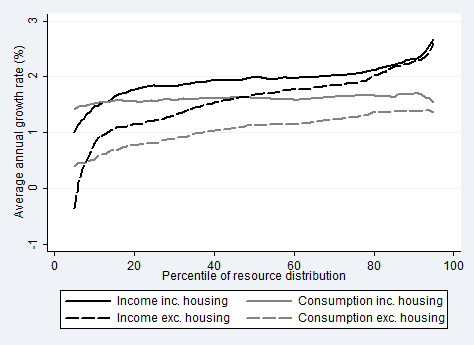
\includegraphics[width=.8\linewidth]{pictures/gic_7.png}
\label{fig:gicall}
\end{figure}

[Needs a note and source. Note that we trimmed the top and bottom 5\%].

\begin{figure}
\caption{Growth Incidence Curves for Income and Consumption, by Sub-Period}
\centering
\begin{tabular}{cc}
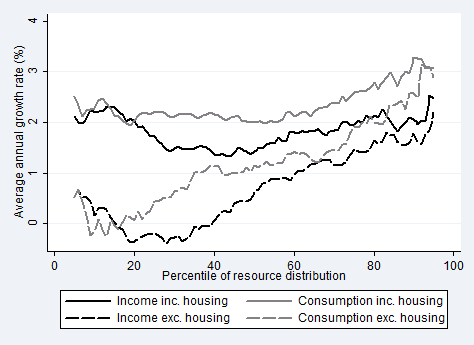
\includegraphics[width=.5\linewidth]{pictures/gic_1.png} & 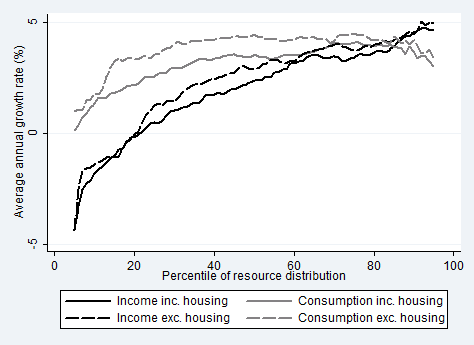
\includegraphics[width=.5\linewidth]{pictures/gic_2.png} \\
(a) 1981-1985 & (b) 1986-1990 \\
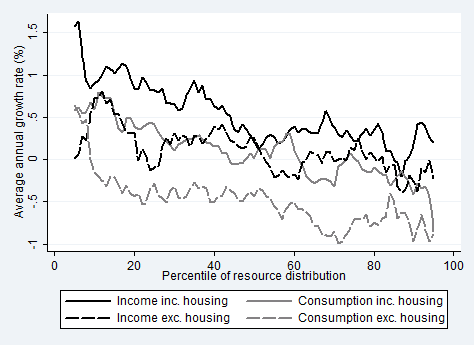
\includegraphics[width=.5\linewidth]{pictures/gic_3.png} & 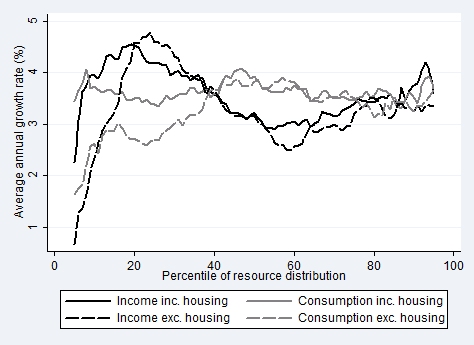
\includegraphics[width=.5\linewidth]{pictures/gic_4.png} \\
(c) 1991-1995 & (d)1996-2000 \\
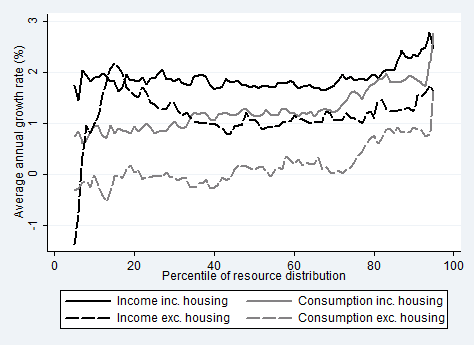
\includegraphics[width=.5\linewidth]{pictures/gic_5.png} & 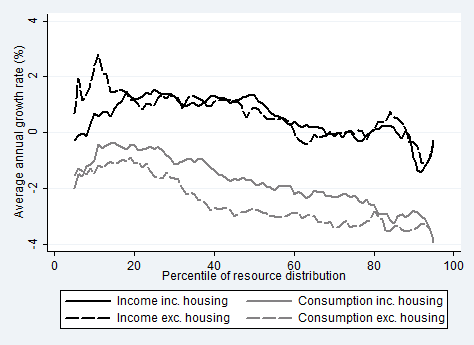
\includegraphics[width=.5\linewidth]{pictures/gic_6.png} \\
(e) 2001-2005 & (f) 2006-2009
\end{tabular}
\label{fig:gicsub}
\end{figure}

[Needs a note and source. Note that we trimmed the top and bottom 5\%].


\begin{figure}
\caption{Average Rooms per Person, 1979-2000}
\centering
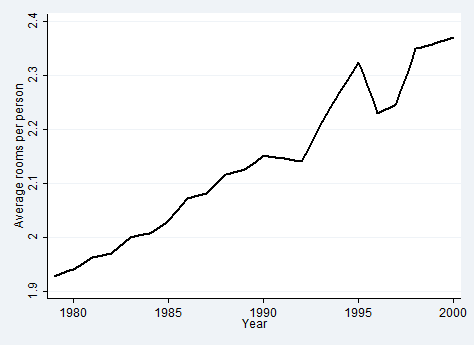
\includegraphics[width=0.7\linewidth]{pictures/rooms_pp.png}
\label{fig:room_time}
\end{figure}


%\newpage

\subsection{Trends in summary measures of inequality and poverty}

%In this sub-section, we explore that the different patterns of growth in household resources, as assessed by our four measures, mean for the evolution of summary measures of inequality and poverty.

Figure \ref{fig:inequal_trends} shows trends between 1979 and 2009 in the 90-10 and 50-10 ratios, and Figure \ref{fig:pov_trends} shows trends in a measure of relative poverty (defined as having a level of resources below 60\% of the contemporaneous median resource measure), for each of the four measure of resources. In general, there was little change in inequality or relative poverty from 1979 to the mid 1980s. As has been well-documented, there was then a sharp rise in inequality and relative poverty, peaking in 1989 or 1990. As we explain in detail shortly, the trends since 1990s depend on the measure used.

As would expected given the difference GICs shown in Figure \ref{fig:gicall}, income and consumption give different impressions of how inequality and poverty have changed between 1979 and 2009.\footnote{In general, trends in the 50-10 ratio are very similar to trends in the relative poverty measure, for all measures of resources.}  First, since the mid 1980s, rates of relative poverty and these measures of inequality have been higher when assessed using income, rather than consumption. In particular, and as suggested by sub-panel (b) of Figure \ref{fig:gicsub}, the rise in inequality and relative poverty in the late 1980s is much more dramatic when assessed with income than with consumption. In measures that do not include imputed resources from housing, inequality and relative poverty have risen faster since 1990 when assessed using consumption than when assessed using income; in measures that do include imputed resources from housing, there has been little difference in the post-1990s trends in inequality in income and consumption.

It is also clear that the measures of resources that do include the imputed resources from housing are more equally distributed, with lower rates of relative poverty and smaller 50-10 ratios, than those that do not, underscoring the fact that the imputed resources derived from housing are more equally distributed than other resources. Furthermore, this inequality-reducing effect of adding the imputed resources from housing is growing over time, so that the post-1990s trends in inequality in resources that do include imputed resources from housing are broadly flat (consumption) or falling (income), but the post-1990s trends in inequality in resources that do not include imputed resources from housing are rising (both income and consumption).


\begin{figure}[bp!]
\caption{Income \& Consumption Inequality, 1979-2009}
\centering
\begin{tabular}{cc}
\multicolumn{2}{c}{90-10 Ratio} \\
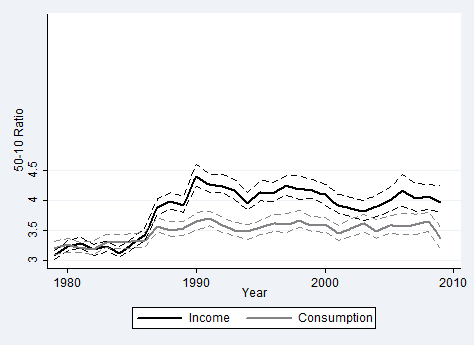
\includegraphics[width=.5\linewidth]{pictures/ihc_1.png} & 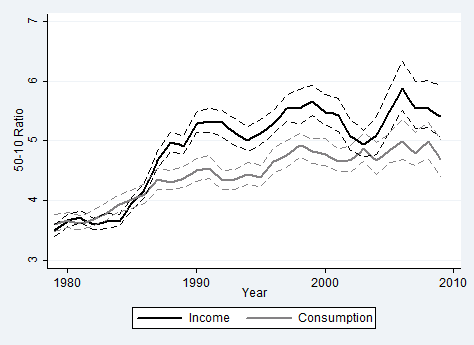
\includegraphics[width=.5\linewidth]{pictures/xhc_1.png} \\
(a) IHC & (b) XHC \\
\multicolumn{2}{c}{50-10 Ratio} \\
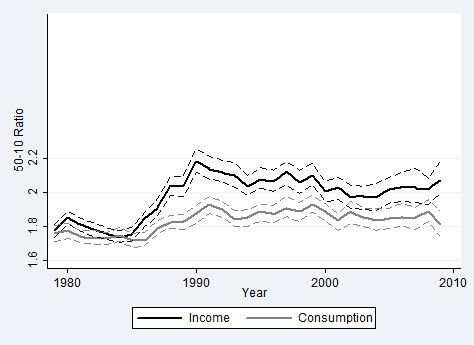
\includegraphics[width=.5\linewidth]{pictures/ihc_2.png} & 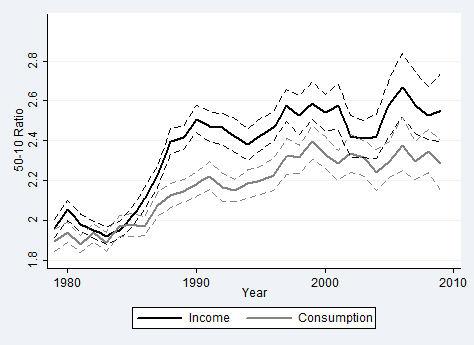
\includegraphics[width=.5\linewidth]{pictures/xhc_2.png} \\
(c) IHC & (d) XHC \\
\end{tabular}
\label{fig:inequal_trends}
\end{figure}

[NEEDS NOTE AND SOURCE. \footnote{Confidence intervals are obtained as $\hat{\mu} + 1.96se(\hat{\mu})$, where $se(\hat{\mu})$ is calculated from the bootstrap distribution of the relevant statistic obtained from 1,000 random draws with replacement independently for each year.}]


\begin{figure}
\caption{Rates of Relative Poverty, 1979-2009}
\centering
\begin{tabular}{cc}
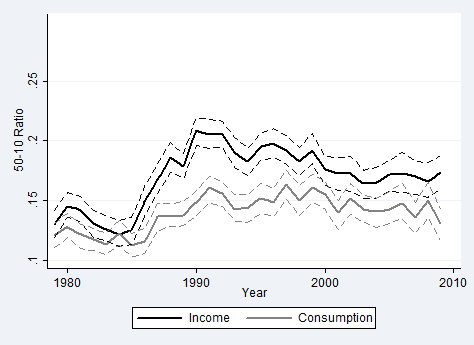
\includegraphics[width=.5\linewidth]{pictures/ihc_3.png} & 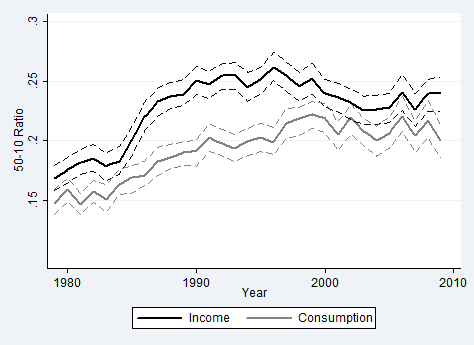
\includegraphics[width=.5\linewidth]{pictures/xhc_3.png} \\
(a) IHC & (b) XHC \\
\end{tabular}
\label{fig:pov_trends}
\end{figure}


[NEEDS NOTE AND SOURCE. \footnote{Confidence intervals are obtained as $\hat{\mu} + 1.96se(\hat{\mu})$, where $se(\hat{\mu})$ is calculated from the bootstrap distribution of the relevant statistic obtained from 1,000 random draws with replacement independently for each year.}]

%\subsection{Summary}
%Overall, this section has shown that conclusions about the rate of growth in household resources, and the evolution of inequality and poverty, are sensitive, for most sub-periods, to the way that resources are measured. Furthermore, the differences in inequality and poverty trends assessed using income and consumption (or between measures that do or do not include imputed resources from housing) cannot be captured simply as an intercept shift. Holding constant the treatment of the imputed resources from housing, the most important of the different impressions one gets when assessing living standards with income and consumption are that resources have grown by more when assessed using income than consumption (particularly in the late 1980s and late 2000s), and that resources have grown in a more unequal way (mostly due to the late 1980s). We have also shown that including the imputed resources from housing increases the rate of growth of household resources - reflecting the growth over time in the ownership of housing, and a trend of having larger housing units - and reduces measures of inequality.




\section{The Composition of the Income-Poor and Consumption-Poor}\label{sec:composition}

The previous section showed that conclusions about the rate of growth in household resources in the UK, and the evolution of inequality and poverty, are sensitive to the way that resources are measured. None of the analysis made use of the fact that our data tells us about income and consumption for the same households. This section examines how income and consumption can give us different impressions of living standards for a given household.  We focus on the extent to which ``having a low income'' and ``having a low consumption'' identify different households, showing that there are a sizeable number of individuals that are classified as ``poor'' when assessed using household income, but not when assessed using consumption measures (and vice versa). We do this for measures that both do and do not include the implicit income or consumption from housing, and Section \ref{sec:housing} then explores that impact the treatment of that implicit income or consumption from housing has on identifying households that are poor.

\subsection{Rank correlations between income and consumption}

%\subsection{The mismatch between the ``income poor'' and the ``consumption poor''}

Table \ref{table:kendall} shows the similarity of the orderings of households given by our four measures of resources by showing the Kendall rank correlation coefficient, $\tau$, for the selection of years shown in Table \ref{table:prctile}.\footnote{For any two pairs of ranks $(x_{i},y_{i})$ and $(x_{j},y_{j})$ of a variable pair $(x, y)$, define them as concordant if: $(x_{i}-x_{j})(y_{i} - y_{j}) > 0$ and discordant otherwise. Kendall's score is then defined as $\tau = \frac{C-D}{\frac{1}{2}n(n-1)}$, where $C$ is the number of concordant pairs and $D$ is the number of discordant pairs.}

Although there is positive agreement between the rankings (i.e. $\tau>0$ for all pairwise comparisons), all measures give different rankings (i.e. $\tau<1$ for all pairwise comparisons). For the measures that do not include imputed resources from housing, $\tau$ has fallen from 0.49 in 1979 to 0.43 in 2009. Unsurprisingly, $\tau$ for the measures that do include imputed resources from housing is slightly higher (reflecting that both measures contain a identical component equal to the imputed resources from housing); more interestingly, it also shows no clear pattern over time, fluctuating between 0.48 and 0.51.

The values of $\tau$ for pairs of measures that do and do not include the imputed income from housing are, unsurprisingly, much higher, but have also fallen over time, from 0.90 to 0.82 for the two measures of income, and from 0.90 to 0.75 for the two measures of consumption. This reflects a rise over time in the implicit resources from housing that is not perfectly aligned with one's position in the without-housing-resources distribution (and this in turn echoes the finding of Figure \ref{fig:gicall} that the inequality-reducing impact of including resources from housing in a measure of consumption is increasing over time.

\begin{table}[tp!]
\caption{Rank Correlation Between Resource Measures: Kendall's Tau}
\centering
\begin{tabular}{lcccc}
\hline\hline 	
 &  Income IHC & Cons. IHC & Income XHC & Cons. XHC \\
\hline
\multicolumn{5}{l}{\textbf{1979}}  \\
Income IHC &1.0000$^{***}$ & & & \\
 & (0.000)  & & & \\
Cons. IHC & 0.4877$^{***}$&1.0000$^{***}$ & & \\
 & (0.000) &(0.000) & & \\
Income XHC & 0.9006$^{***}$&0.4716$^{***}$ &1.0000$^{***}$ & \\
  & (0.000) &(0.000) & (0.000) & \\
Cons. XHC &0.4733$^{***}$ &0.8980$^{***}$ &0.4890$^{***}$ &1.0000$^{***}$ \\
 & (0.000) &(0.000) & (0.000) & (0.000) \\
\hline
\multicolumn{5}{l}{\textbf{2009}}  \\
Income IHC &1.0000$^{***}$ & & & \\
 & (0.000)  & & & \\
Cons. IHC & 0.4755$^{***}$&1.0000$^{***}$ & & \\
 & (0.000) &(0.000) & & \\
Income XHC & 0.8202$^{***}$&0.3956$^{***}$ &1.0000$^{***}$ & \\
  & (0.000) &(0.000) & (0.000) & \\
Cons. XHC &0.4066$^{***}$ &0.7574$^{***}$ &0.4281$^{***}$ &1.0000$^{***}$ \\
 & (0.000) &(0.000) & (0.000) & (0.000) \\
\hline\hline
\multicolumn{5}{l}{Notes: p-values in brackets. }
\end{tabular}
\label{table:kendall}
\end{table}

\subsection{New title?}

To probe to what extent the different rank correlations are relevant for the low-income population, Figure \ref{fig:overlap} shows trends in the proportion of the population who are in both the bottom decile group of the distribution of income and the distribution of consumption (and calculated separately for measures that do and do not include imputed resources from housing). A perfect rank correlation between a pair of measures would means that this fraction would be 10 percent. However, the average proportion of the population in the bottom decile groups of both of the distributions that do not include imputed income from housing was 2.32\% between 1979 and 2009.\footnote{Although not shown here, the degree of overlap is even lower when one considers all four measures simultaneously: averaged over each year in our data, only 1.69\% of the population was in the bottom decile group of all four resource distributions on average.} For the distributions of the resources that do included imputed resources from housing, this was higher, at 3.96\%, and is on an increasing trend. As before, the fact that the fraction deemed poor on both income and consumption is higher when we include imputed resources from housing than when we do not reflects that the two measures that include imputed resources from housing are (weakly) positively correlated by construction, and the fact that the fraction deemed poor on both is rising over time when using a resource measure that includes imputed resources from housing reflects that the imputed income from housing is growing in importance at the bottom of the resource distribution.


\begin{figure}
\caption{In Bottom Decile of Income and Consumption Distributions}
\centering
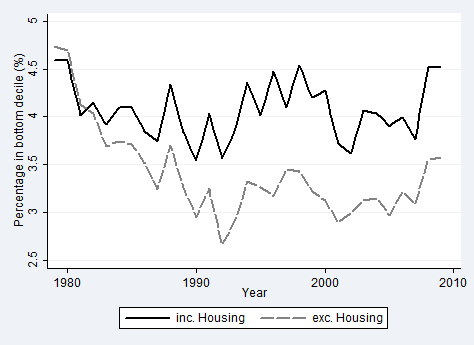
\includegraphics[width=.7\linewidth]{pictures/overlap.png}
\label{fig:overlap}
\end{figure}

\subsection{New title?}
As income and consumption do, then, give different orderings of households and identify different households as having low resources, it is worth assessing which measure better correlates with other indicators of low living standards. We proceed using an approach suggested by \citet{meyer2003measuring}.
We define four groups $BrInc_{low}$. $BrInc_{notlow}$, $Con_{low}$
and $Con_{notlow}$, where the subscript `low' refers to those households
lying in the bottom 10 per cent of the consumption or income distribution,
and `notlow' to those households lying in the upper 90 per cent of
the distribution in question, and BrInc
and Con refer to broad income and consumption respectively. Defining
$X$ as some outcome that (at least arguably) correlates positively
with living standards (for example having health insurance or owning
one's own home), and defining $X(y)$ as the mean outcome for group
$y$, we then calculate a difference-in-difference type measure:

\begin{equation}
\left[X(Con_{low})-X(Con_{notlow})] - [X(BrInc_{low})-X(BrInc_{notlow})\right]\label{eq:diffindiff}
\end{equation}


This will be negative if being in the bottom decile group of reported
consumption is a better indicator of poor outcomes than being in the
bottom decile group of reported income.

We calculate this measure for ownership of various consumer durables
(dishwasher, washing machine, central heating, computer, DVD player,
access to the internet at home, a TV, subscription TV), having health
insurance, owning one or more cars, owning their own house, and the
number of rooms in the house. We noted above that the measure of consumption
used here does not include any spending on durables. This is to avoid
the generation of mechanical (and not particularly informative) relationships
between the measure of consumption and ownership of durables.

The results are shown in Table \ref{tab:Rel_cons_inc_all}. All but
one of the statistics have a negative sign and are statistically significant;
the exception is owning a TV (perhaps unsurprisingly as the vast majority
of all households now own a TV). Although the LCFS provides
a limited number of alternative measures of living standards, overall
we conclude emphatically that having a low recorded consumption is
a better guide to who has a low living standard than having a low
reported income.

% Table generated by Excel2LaTeX from sheet 'Table 6'
\begin{sidewaystable}
%\begin{table}[htbp]
\centering
\caption{The relationship between low consumption, low income and other outcomes, all households}
\begin{tabular}{lcccccccc}
\addlinespace
\toprule
& (1)    & (2)    & (3)    & (4)    & (5)    & (6)    & (7)    & N \\
\midrule
& $X(Inc_{low})$ & $X(Inc_{notlow})$ & (1)-(2) & $X(Con_{low})$ & $X(Con_{notlow})$ & (4)-(5) & (6)-(3) &  \\
Wsh. Mch. & 0.92  & 0.96  & -0.04 & 0.84  & 0.96  & -0.12 & -0.083*** & 52,796 \\
Cent. Heat. & 0.92  & 0.94  & -0.03 & 0.89  & 0.95  & -0.06 & -0.030*** & 52,796 \\
Dishwash. & 0.20   & 0.36  & -0.16 & 0.06  & 0.37  & -0.31 & -0.151*** & 52,796 \\
DVD   & 0.59  & 0.61  & -0.03 & 0.42  & 0.63  & -0.22 & -0.189*** & 52,796 \\
TV    & 0.98  & 0.99  & -0.01 & 0.98  & 0.99  & -0.01 & 0.002 & 52,796 \\
Pay TV & 0.30   & 0.39  & -0.09 & 0.18  & 0.40   & -0.22 & -0.134*** & 52,796 \\
PC    & 0.54  & 0.64  & -0.10  & 0.24  & 0.68  & -0.44 & -0.335*** & 52,796 \\
Internet & 0.41  & 0.56  & -0.15 & 0.15  & 0.59  & -0.44 & -0.286*** & 52,796 \\
Car   & 0.53  & 0.78  & -0.25 & 0.24  & 0.82  & -0.57 & -0.321*** & 52,796 \\
Two cars & 0.14  & 0.33  & -0.19 & 0.02  & 0.34  & -0.32 & -0.130*** & 52,796 \\
Own hse. & 0.37  & 0.74  & -0.38 & 0.32  & 0.75  & -0.43 & -0.055*** & 52,796 \\
No. rooms & 4.97  & 5.38  & -0.41 & 4.5   & 5.44  & -0.94 & -0.528*** & 52,796 \\
Health ins. & 0.05  & 0.13  & -0.08 & 0.02  & 0.13  & -0.12 & -0.036*** & 52,796 \\
\bottomrule
\multicolumn{9}{c}{\parbox[b]{18cm}{
{\footnotesize{Source: Authors' calculation using Expenditure and Food Survey/Living Costs and Food Survey 2001/02- 2009. \\*
Notes: Column (7) gives the quantity expressed in equation (3). Negative numbers indicate that consumption is better correlated with the outcome in the left-hand column (e.g. having a washing machine, owning one's own home) than is income. Other columns give the individual components of the quantity in equation (3). *** indicates significant at the 1\% level, ** indicates significant at the 5\% level, * indicates significant at the 10\% level. Confidence intervals are calculated by bootstrapping with 999 replications.}}}}
\end{tabular}%
\label{tab:Rel_cons_inc_all}%
%\end{table}%
\end{sidewaystable}%


\subsection{New title?}
%Given the differences in ranking between resource distributions, there are a number of individuals for whom resource distribution matters for whether they are identified as having low living standards: they would be classed as living in poverty if their living standards were measured using income but not if they were measured by consumption and vice versa. It is informative to dig deeper into differences in the characteristics of the individuals who make up the bottom deciles of the different resource distributions.

%We begin with a simple descriptive analysis.
We now examine the composition of the bottom of each of the income and consumption distribution. Indeed, analysis such as this is extremely relevant for those interested in designing policies targeted at those with a low living standard.

We begin with a relatively simple breakdown, asking to what extent individuals with the lowest resources are the elderly, or are children. Figure \ref{fig:age_comp} shows, in each year and for each of our four measures of household resources, the proportion of the bottom decile group who are working-age adults (panel (a)) and the elderly [Mike asks Abi: how define ``pensioners'' or the ``elderly''?] (panel (b)), with children representing the omitted category.

There is a consistent story across all measures that the proportion of the bottom decile group who are pensioners is considerably lower in 2009 than it was in 1979. [LINK TO OTHER WORK.] But the extent to which the group deemed to have low resources contains the elderly depends on how resources are measured. Two facts are clear. First, regardless of the treatment of resources from housing, the proportion of the bottom decile group who are pensioners is lower when assessed using income than when using consumption.\footnote{Crossley and O'Dea (2010) present an analysis that is consistent with this finding by showing the median saving rate (defined as \emph{income less spending} as a fraction of \emph{income} by age that is implied by the same LCFS data as we analyse here. These implied saving rates rise strongly with age for those aged over 60; equivalently, many elderly households report in the LCFS cash spending levels that are considerably lower than their cash income. This seems counter-intuitive, at least if one has in mind a simple lifecycle model of asset accumulation and decumulation. Finch and Kemp (2006), analysing the same data that we use, concluded that ``although the evidence has been far from conclusive, low spending amongst pensioner households appears to reflect an inter-related set of factors associated with increasing frailty and declining mobility, leading to reducing social participation and contracting social networks.'' Put more crudely, they found no evidence that the data was under-recording spending, and attributed the low levels of spending to a declining ability (or need) to spend money as older people's health deteriorated. Using qualitative research, Dominy and Kempson (2006) found considerable evidence of saving going on amongst the elderly, much of which would probably be considered by economists as precautionary saving for unexpected, lumpy items of spending. In the absence of high-quality longitudinal data on household wealth, more research is needed before we can conclude whether the LCFS is offering a correct impression of the savings behaviour of the elderly, and if so, what economic explanation lies behind it. Until, we need to be mindful that income and consumption do give differing impressions of the living standards of the elderly in ways which may be different from conventionally assumed. We will return to this discussion in Section \ref{sec:housing}.[Mike notes: yes I know it's a big footnote. Abi has this material in the text later on, but I think a mention of it needs to come here. Or do we need to put this in the main text and make more of it?]}. Second, moving to a measures of resources that includes imputed resources from housing reduces the proportion of the bottom decile group who are pensioners (particularly when using consumption). In the first two cases, the opposite is true for the  proportion who are working-age adults, for the last case, the same is also true for the proportion who are working-age adults, implying that moving to a measures of resources that includes imputed resources from housing increases the proportion of the bottom decile group who are children.

\begin{figure}
\caption{Age Composition of Bottom Decile Group of Income and Consumption}
\centering
	\subfloat[Working age]
	{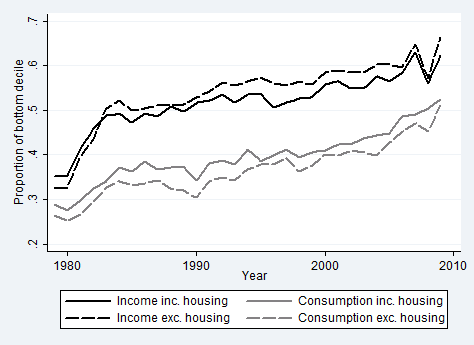
\includegraphics[width=.5\linewidth]{pictures/dec_comp2.png}} \\
	\subfloat[Pensioners]
	{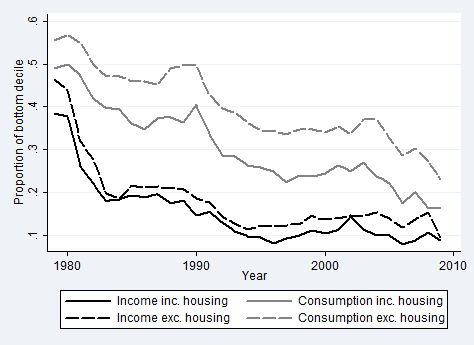
\includegraphics[width=.5\linewidth]{pictures/dec_comp3.png}} \\
	\subfloat[Children]
	{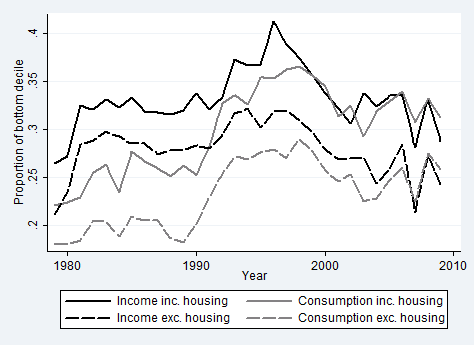
\includegraphics[width=.5\linewidth]{pictures/dec_comp1.png}} \\
\label{fig:age_comp}
\end{figure}

Figure \ref{fig:pov_comp} shows the proportion of the bottom decile group with low levels of educational qualifications (defined as leaving school at, or younger than, 16 years old). The most striking finding is the stark change over time whereby the bottom decile group (however measured) has become increasingly well educated. However, what is more interesting is that those with a low consumption are more likely to be low educated compared to those with a low income. Because we would expect levels of education to be strongly correlated with levels of resources (including those coming from housing) assessed over a lifetime, then this suggests that identifying the poor using low consumption is better at identifying those more likely to be long-term poor than using income, as does using a measure that includes the imputed resources from housing.

\begin{figure}
\caption{Proportion of More Educated Individuals in Bottom Decile Group of Income and Consumption}
\centering
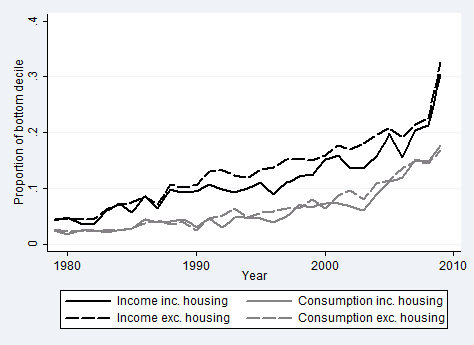
\includegraphics[width=.7\linewidth]{pictures/dec_comp4.png}
\label{fig:pov_comp}
\end{figure}

We now probe this suggestion further by testing the significance of observed demographic factors as predictors of having a low living standard assessed using both income and consumption. To do this, we estimate a multinomial logit model with four outcome categories: (1) in the bottom decile group of both income and consumption resource distributions; (2) in the bottom decile group of the income distribution but not the consumption distribution; (3) in the bottom decile group of the consumption distribution but not the income distribution; (4) not in the bottom decile group of either the income and consumption distributions. With ``not in the bottom decile group of either the income and consumption distributions'' as the reference category, we then test for equality of the relative risk ratios that correspond to a given demographic characteristic.\footnote{An alternative approach would be to estimate separate logits for being in the bottom decile group of income and of consumption, and comparing coefficients across models. However, as noted in Allison (1999), coefficients in binary regression are confounded with residual variation, and so differences in the amount of residual variation between groups can produce differences in slope coefficients between groups that are not indicative of causal differences. Although solutions have been proposed to deal with this problem, all have their drawbacks (see, for example, Williams (2009) and Mood (2010)) and there is yet no consensus. We therefore we estimate a multinomial logit model and test for significant differences in the impact that characteristics have in predicting income-only-poverty versus consumption-only-poverty. If a characteristic was just as effective at predicting income-poverty as it was consumption-poverty - which is the interpretation that people like to make when logit coefficients are found to be equal to each other - then these relative risk ratios in our multinomial logit should not be significantly different from each other.}

The results are in Table \ref{table:multinom_incon}, which shows the relative risk ratios of several demographic characteristics for the outcomes ``in the bottom decile group of both income and consumption resource distributions'', $r_{IC}$, ``in the bottom decile group of the income distribution but not the consumption distribution'', $r_{I}$, and ``in the bottom decile group of the consumption distribution but not the income distribution'', $r_{C}$.  The key parameter of interest, reported in the column titled $r_{I}-r_{C}$, is then the difference between the relative risk ratio of being ``in the bottom decile group of the income distribution but not the consumption distribution'' and ``in the bottom decile group of the consumption distribution but not the income distribution'', and we report the $\chi^{2}$ test statistic for their equality. Note that a negative (positive) value in the $r_{I}-r_{C}$ column means that that demographic characteristic is a better predictor of having a low consumption than it is for having a low-income. \footnote{The results given here are for the sub-period 1999-2009. The results for earlier decades show the same qualitative story, and can be found in the Appendix \ref{sec:annex_results}.}

To give an illustration of how to interpret this, recall that Figure \ref{fig:pov_comp} showed that the bottom decile group of the consumption distribution contained more low-educated individuals than the bottom decile group of the income distribution, meaning that having a low education is a better predictor of having a low consumption than it is of having a low income. This is reflected in the left-hand panel of Table \ref{table:multinom_incon}, where there is a higher relative risk ratio on ``left school $\leq16$'' in column $r_{C}$ (2.460) than there is in column $r_{I}$ (1.300). The fourth column of the left-hand panel, $r_{I}-r_{C}$, reports the difference in these relative risk ratios, confirming that it is negative, and statistically different from zero at the 5\% level. The interpretation is, therefore, that  having a low education is more strongly correlated with having a low consumption than having a low income.

Looking at all rows of Table \ref{table:multinom_incon}, the left-hand panel shows that the risk of being in the bottom decile group of the income distribution but not of the consumption distribution is higher for those who are under 30, highly educated, and unemployed, and, conversely, the risk of being in the bottom decile group of the consumption distribution but not of the income distribution is higher for those who over 60, have low education, and who are not unemployed.  Finally, the left-hand panel of the table repeats the analysis but using measures of income and consumption that do not add resources from housing. The conclusions are very similar: the risk of being in the bottom decile group of the income distribution but not of the consumption distribution where we do not add resources from housing is higher for those who under 30, highly educated, and unemployed.

\begin{sidewaystable}
\caption{Demographics and the Bottom Decile, 1999-2009: Multinomial Logit Relative Risk Ratio [Mike asks Abi and Cormac: can you provide a more informative or descriptive title]}
\centering
\begin{tabular}{l|cccc|cccc}
\hline\hline
	& \multicolumn{4}{c}{\textbf{IHC Bottom Decile}} &  \multicolumn{4}{c}{\textbf{XHC Bottom Decile}} \\
	&	Inc \& Cons.	&	Inc. Only	&	Cons. Only	&	Diff.	&	Inc \& Cons	&	Inc Only	&	Cons. Only	&	Diff. 	\\
	&	$r_{IC}$	&	$r_{I}$	&	$r_{C}$ &	$r_{I}$-$r_{C}$&	$r_{IC}$	&	$r_{I}$	&	$r_{C}$	&	$r_{I}$-$r_{C}$\\
 & se & se & se & $\chi^{2}$  & se & se & se & $\chi^{2}$ \\
\hline
Left school $\leq$ 16	&	       2.370***	&	       1.20***	&	       2.68***	&	-1.48***	&	     					  1.47*** 	&	1.07	&	       2.21***	&	-1.14***	\\
                    	&	       0.252   	&	0.09	&	0.28	&	58	
		&	       0.088   	&	0.06	&	0.15	&	55	\\
Left school $>$ 19	&	       1.71***   	&	       0.92  	&	       0.99* 	&	-0.07	&
				       0.85*   	&	0.94	&	0.96	&	-0.02	\\
                    	&	       0.177   	&	0.07	&	0.11	&	0.25	&	
			      0.069   	&	0.09	&	0.07	&	0.05	\\
Age $<$ 30	&	       1.150   	&	       1.55***	&	1.32***	&	0.23***	&
			       1.21*   	&	       1.36***	&	1.25***	&	0.10	\\
                    	&	       0.142   	&	0.11	&	0.12	&	4.51	&	
			       0.133   	&	0.08	&	0.10	&	1.9	\\
Age 30-40	&	       1.032   	&	1.14**	&	       1.11** 	&	0.03	&	
			       0.85***	&	1.02	&	1.09***	&	-0.07	\\
                    	&	       0.068   	&	0.07	&	0.05	&	0.12	&	
			       0.047   	&	0.05	&	0.05	&	0.64	\\
Age 50-60	&	       0.791**  	&	       0.85*** 	&	0.96	&	-0.11	&
			       0.91   	&	       0.82***  	&	1.02	&	-0.20***	\\
                    	&	       0.093   	&	0.04	&	0.03	&	3.22	&	
			       0.055  	&	0.04	&	0.06	&	7.00	\\
Age 60-70	&	       0.263***	&	       0.41***	&	       1.00 	&	-0.59***	&	       						0.14***	&	       0.36***	&	1.10	&	-0.74***	\\
                    	&	       0.034   	&	0.04	&	0.08	&	46.51	&	
			    0.012   	&	0.03	&	0.07	&	113	\\
Age $\geq$ 70	&	       0.331***	&	       0.20***	&	       2.12***	&	-1.92***	&	       					0.20***	&	       0.21***	&	       2.46***	&	-2.25***	\\
                    	&	       0.051   	&	0.02	&	0.18	&	284	&	       0.03   	&	0.01	&	0.24	&	445	\\
Workless	&	       13.130***	&	       6.57***	&	       3.17***	&	3.41***	&	       						17.2***	&	       7.54***	&	       3.54***	&	4.00***	\\
	&	1.33	&	0.52	&	0.26	&	42	&	
	1.43	&	0.38	&	0.18	& 	82 \\
Self Employed	&	       13.130***	&	       3.88***	&	       0.92 &	2.96***	&	       							1.64***	&	       4.23***	&	       0.89 &	3.34***	\\
	&	1.33	&	0.35	&	0.08	&	88	&
		0.20	&	0.37	&	0.09		& 121	\\
Couple	&	      0.776***	&	       0.85***	&	      0.72***	&	0.13**	&	       						0.96	&	      1.11	&	      0.93	&	0.19**	\\
			&	0.069	&	0.08	&	0.05	&	5.5	&
			0.07	&	0.10	&	0.06		&4.3	\\
Single	&	     0.993	&	       1.14	&	      0.90	&	0.24**	&
		       3.43***	&	       2.22***	&	       2.42***	&	-0.21	\\
	&	0.101	&	0.12	&	0.07	&	6.5	&
		0.280	&	0.19	&	0.17		& 0.9	\\
Children	&	      2.707***	&	       1.53***	&	       2.63***	&	-1.10***	&	       					0.85***	&	       1.12	&	       1.81***	&	-0.69***	\\
	&	0.234	&	0.12	&	0.09	&	124	&	
		0.066	&	0.08	&	0.06		& 55	\\
Constant            	&	       0.013***	&	       0.056***	&	       0.085***	&		&	      					 0.02***	&	       0.069***	&	       0.074***	&		\\
                    	&	       0.00   	&	0.01	&	0.01	&		
		&	       0.00   	&	0.01	&	0.01	&		\\
\hline\hline
\multicolumn{9}{l}{Significantly different from zero at the  10\% ($\star$), 5\% ($\star\star$) and 1\% level ($\star\star\star$).} \\
\multicolumn{9}{l}{Omitted variables: Left school between 17-18 years old, household head aged between 40 and 50 years, employed. }
\end{tabular}
\label{table:multinom_incon}
\end{sidewaystable}


%\subsection{Need title?}

Overall, the results reported in Table \ref{table:multinom_incon} provides further weight for our hypothesis that those found at the bottom of the income distribution are those who are more likely to be temporarily poor - the young, those with high levels of education, and the unemployed (who will presumably soon become employed - than those found at the bottom of the income distribution. [Mike says: although I note that there is an issue with age, and the non-spending older people. REFER BACK TO EARLIER DISCUSSION].

We explore this further in Table \ref{table:interact}, which now interacts age, education and unemployment. Focusing on the  $r_{I}-r_{C}$ column in the left-hand panel, the results show that those characteristics that are more associated with being consumption-poor than income-poor are: having a low education, and being aged over 60. Being out of work is more associated with being income-poor than being consumption-poor, and especially so for those aged under 30, but this effect is reduced for those who are both low-education and unemployed, or aged over 60 and unemployed. As above, if we think of those who are young and out-of-work as more likely to be in a position of temporary low income than those who are older and out-of-work, and similarly for those with high levels of education compared to those with low levels of education, then having a low consumption seems more likely to identify those individuals who are at greater risk of long-term poverty.\footnote{Results in the right-hand panel are qualitatively identical.}


\begin{sidewaystable}
\caption{Age, Education \& Unemployment, 2000-2009: Multinomial Logit Relative Risk Ratio}
\centering
\begin{tabular}{l|cccc|cccc}
\hline\hline
	& \multicolumn{4}{c}{\textbf{IHC Bottom Decile}} &  \multicolumn{4}{c}{\textbf{XHC Bottom Decile}} \\
	&	Inc \& Cons.	&	Inc Only	&	Cons. Only	&	Diff.	&	Inc \& Cons	&	Inc Only	&	Cons. Only	&	Diff. 	\\
	&	$r_{IC}$	&	$r_{I}$	&	$r_{C}$ &	$r_{I}$-$r_{C}$&	$r_{IC}$	&	$r_{I}$	&	$r_{C}$	&	$r_{I}$-$r_{C}$\\
 & se & se & se & $\chi^{2}$  & se & se & se & $\chi^{2}$ \\
\hline
Left school $\leq$ 16	&	       2.63***	&	       1.32***	&	       2.25***	&	-0.92***	&	       						1.20   	&	       1.20***  	&	      1.96***	&	-0.75***	\\
                    				&	       0.43   	&	0.09	&	0.21	&	21	&	
			      				 0.18   	&	0.08	&	0.17	&	20	\\
Left school $>$ 19	&	       1.13   	&	       0.71***	&	       0.81*** 	&	-0.10	&	       						0.62**   	&	       0.82** 	&	0.93	&	-0.12	\\
                   	 	&	       0.23   	&	0.06	&	0.10	&	0.80	&	
			  	   0.12   	&	0.06	&	0.10	&	1.00	\\
Workless*Left school $\leq$ 16	&	       0.90   	&	0.86	&	       1.39**  	&	-0.53***	&	       					1.27  	&	       0.82**  	&	1.021	&	-0.39***	\\
                    	&	       0.17   	&	0.09	&	0.19	&	8.7	&
	       0.22   	&	0.08	&	0.14	&	7.4	\\
Workless*Left school $>$ 19	&	       2.10***   	&	       1.96***	&	1.48**	&	0.49	&	       1.63 **  	&	       1.39***	&	1.01	&	0.38***	\\
	&	       0.50   	&	0.25	&	0.28	&	1.7	&
	       0.37   	&	0.17	&	0.16	&	3.0	\\
Age $<$ 30	&	       1.30*  	&	       1.62*** 	&	1.35***	&	0.27	&	
			       1.07   	&	1.25***	&	1.27**	&	-0.02	\\
	&	       0.20   	&	0.15	&	0.14	&	1.8	&	
			    0.19  	&	0.11	&	0.13	&	0.01	\\
Age 30-40	&	       0.85   	&	1.11	&	       1.132 	&	-0.02	&	
			       0.78  	&	      0.97  	&	1.08	&	-0.11	\\
                    	&	       0.11  	&	0.08	&	0.09	&	0.03	&	
			       0.13   	&	0.06	&	0.09	&	1.12	\\
Age 50-60	&	       0.70**  	&	0.84**	&	0.82**	&	0.02	&	
			       0.95   	&	       0.81***  	&	0.99	&	-0.18	\\
                    	&	       0.12  	&	0.07	&	0.08	&	0.04	&	
			       0.16   	&	0.06	&	0.10	&	2.7	\\
Age 60-70	&	       0.47** 	&	0.72***	&	       1.245**	&	-0.52***	
		&	       0.42*** 	&	       0.62***	&	1.28	&	-0.66***	\\
                    	&	       0.14   	&	0.09	&	0.17	&	5.32	&	
			       0.13   	&	0.07	&	0.16	&	20	\\
Age $\geq$ 70	&	       0.34***	&	       0.18***	&	       1.99***	&	-1.81***	&	       						0.21***	&	       0.21***	&	       2.29***	&	-2.08***	\\
                    	&	       0.03   	&	0.02	&	0.17	&	452	&	
			      0.02   	&	0.02	&	0.18	&	573	\\
Workless*Age $<$ 30	&	       0.87   	&	0.82	&	0.84	&	-0.102
				&	       1.23   	&	1.16	&	0.91	&	0.25	\\
				&	       0.16  	&	0.11	&	0.13	&	0.03	&	
					   0.25   	&	0.15	&	0.14	&	2.0	\\
Workless*Age 30-40	&	       1.30*   	&	1.03	&	0.93	&	0.10	&	
				       1.11   	&	1.14	&	0.97	&	0.17	\\
			&	       0.20   	&	0.12	&	0.12	&	0.44	&	
				      0.20   	&	0.12	&	0.12	&	1.3	\\
Workless*Age 50-60	&	       1.15  	&	0.95	&	1.28	&	-0.32	&	
				       0.93   	&	0.97	&	1.01	&	-0.04	\\
			&	       0.22   	&	0.11	&	0.18	&	2.9	&	
				   0.17   	&	0.10	&	0.13	&	0.1	\\
Workless*Age 60	&	       0.52**   	&	       0.47***	&	       0.73**  	&	-0.26**	&	
			   0.31***	&	       0.52***	&	0.77	&	-0.25**	\\
	&	       0.17   	&	0.06	&	0.11	&	4.7	&	
		       0.09   	&	0.07	&	0.11	&	4.6	\\
Workless	&	       11.8***	&	       7.22***	&	       2.48***	&	4.73***	
		&	       13.9***	&	       8.14***	&	       3.30***	&	4.85***	\\
		&	       2.40   	&	0.84	&	0.37	&	35	
		&	       2.61   	&	0.87	&	0.44	&	32	\\
Self emp	&	       1.30*	&	       3.80***	&	      0.91	&	2.89***	
		&	       1.52**	&	       4.09***	&	       0.91 &	3.18***	\\
		&	       0.19   	&	0.22	&	0.09	&	166	
		&	       0.26   	&	0.22	&	0.09	&	184	\\
Couple	&	       0.84**	&	      0.91	&	     0.75**	&	0.16***	
		&	       1.02	&	       1.16**	&	      0.98	&	0.18**	\\
		&	       0.07   	&	0.05	&	0.05	&	5.8	
		&	       0.10   	&	0.07	&	0.06	&	4.3	\\
Single	&	       1.06	&	       1.23*** 	&	   0.93	&	0.30***	
		&	       3.66***	&	     2.32***	&	       2.52***	&	-0.21	\\
		&	       0.08   	&	0.07	&	0.06	&	12	
		&	       0.31   	&	0.13	&	0.16	&	1.1	\\
Children	&	       2.68***	&	     1.52***	&	      2.65***	&	-1.13***	
		&	       0.86***	&	      1.10**	&	       1.83***	&	-0.73***	\\
		&	       0.17   	&	0.07	&	0.15	& 67	
		&	       0.05   	&	0.05	&	0.10	& 64	\\
Constant            	&	       0.01***	&	       0.04***	&	       0.03***	&		&	       0.02***	&	       0.04***	&	       0.03***	&		\\
                    	&	       0.002   	&	0.004	&	0.001 	&		&	       0.003   	&	0.004	&	0.003	&		\\
\hline\hline
\multicolumn{9}{l}{Significantly different from zero at the 10\% ($\star$), 5\% ($\star\star$) and 1\% level ($\star\star\star$).} \\
\multicolumn{9}{l}{Omitted variables: Left school between 17-18 years old, household head aged between 40 and 50 years, employed. }
\end{tabular}
\label{table:interact}
\end{sidewaystable}



\subsection{Summmary}

In summary, we have shown that [...].

\section{How important is the treatment of resources from housing in determining who is poor?}\label{sec:housing}

Previous sections have shown that conclusions about the rate of growth in household resources, and the evolution of inequality and poverty, are sensitive, for most sub-periods, to the way that resources are measured. Section \ref{sec:trends} showed that adding the imputed resources from housing to our measure of household resources increases the impression of by how much living standards have grown over the past 30 years, and reduces measures of inequality. This section explores how adding the imputed resources from housing changes our impression of which households are in poverty, in a similar way to how Section \ref{sec:compositionwith} explored how income and consumption identified different groups of households as being in poverty. [And does something else too?]

\begin{figure}
\caption{Risk of Poverty, by Age and Cohort }
\centering
\begin{tabular}{c c}
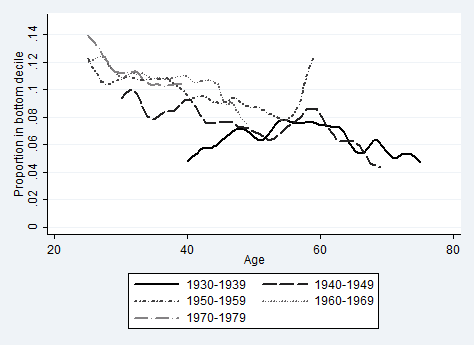
\includegraphics[width=.5\linewidth]{pictures/cohortagerisksmooth_bhc_inc.png} &
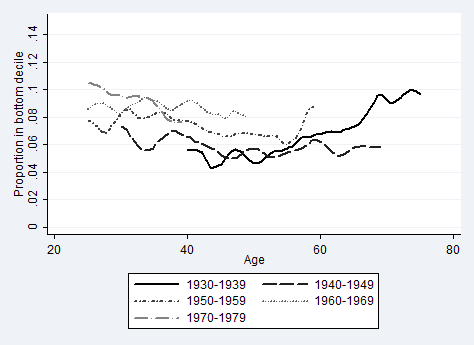
\includegraphics[width=.5\linewidth]{pictures/cohortagerisksmooth_bhc_con.png} \\
(a) Income inc. Housing & (b) Consumption inc. Housing \\
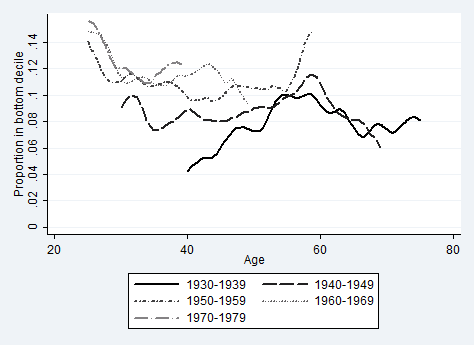
\includegraphics[width=.5\linewidth]{pictures/cohortagerisksmooth_ahc_inc.png} &
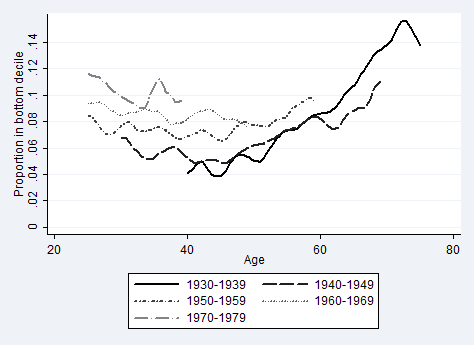
\includegraphics[width=.5\linewidth]{pictures/cohortagerisksmooth_ahc_con.png} \\
(c) Income ex. Housing & (d) Consumption ex. Housing \\
\end{tabular}
\label{fig:povage_cohort}
\end{figure}

\begin{figure}
\caption{Risk of Poverty, by Age and Cohort }
\centering
\begin{tabular}{c c}
Income & Consumption\\
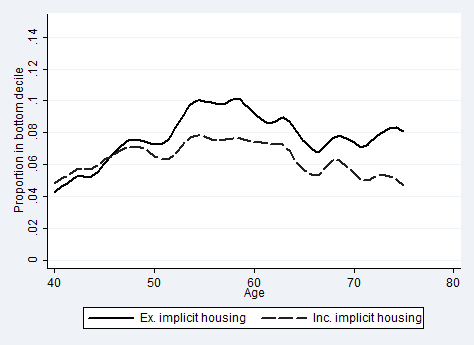
\includegraphics[width=.5\linewidth]{pictures/cohort2_agerisksmooth_inc.png} &
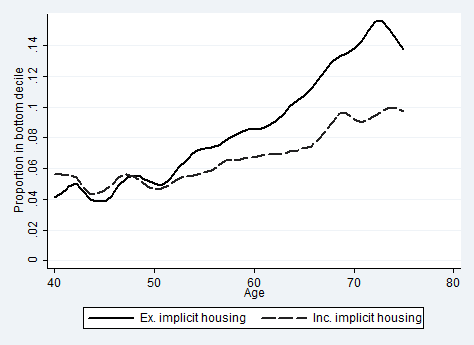
\includegraphics[width=.5\linewidth]{pictures/cohort2_agerisksmooth_con.png} \\
(a) 1930s Cohort & (b) 1930s Cohort \\
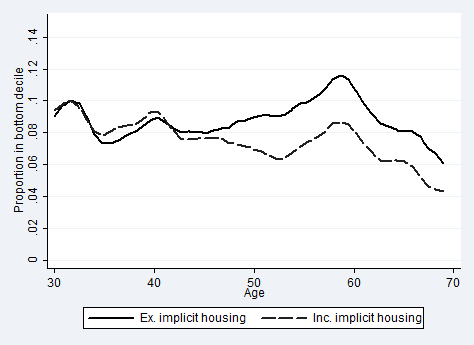
\includegraphics[width=.5\linewidth]{pictures/cohort3_agerisksmooth_inc.png} &
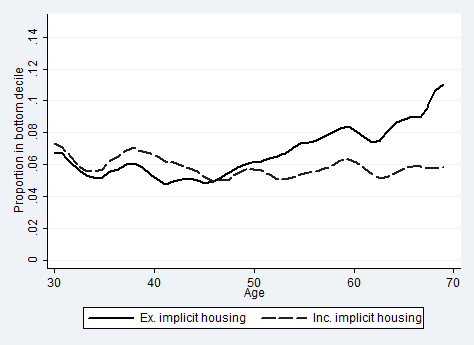
\includegraphics[width=.5\linewidth]{pictures/cohort3_agerisksmooth_con.png} \\
(c) 1940s Cohort & (d) 1940s Cohort \\
\end{tabular}
\label{fig:povage_cohort_restrict}
\end{figure}

\begin{sidewaystable}
\caption{Demographics and the Bottom Decile of IHC \& XHC Distributions, 1999-2009: Relative Risk Ratios}
\centering
\begin{tabular}{l|cccc|cccc}
\hline\hline 
	& \multicolumn{4}{c}{\textbf{Income Bottom Decile}} &  \multicolumn{4}{c}{\textbf{Cons. Bottom Decile}} \\
	&	$r_{IX}$	&	$r_{I}$	&	$r_{X}$ &	$r_{I}$-$r_{X}$&	$r_{IX}$	&	$r_{I}$	&	$r_{X}$	&	$r_{I}$-$r_{X}$\\
  & se & se & se  & $\chi^{2}$ & se & se & se & $\chi^{2}$ \\
\hline
Left school $\leq$ 16	&	       1.37***  	&	       2.51***	&	      1.45***	&	1.06****	&	     					  3.17***	&	       2.89***	&	2.79***	&	0.11	\\
                   		 	&	       0.10  	&	0.31	&	0.09	&	18	&	      
						 0.23   	&	0.33	&	0.27	&	0.08	\\
16 $<$ Left school $<=$ 19	&	       0.96   	&	       0.97  	&	1.46***	&	-0.48***	&	
				       1.08   	&	       1.01  	&	       1.78***  	&	-0.78***	\\
                    		&	       0.08   	&	0.09	&	0.14	&	7.8	&	     
					  0.08   	&	0.09	&	0.18	&	24	\\
Age $<$ 30	&	       1.92*** 	&	       1.89***  	&	1.95***	&	-0.06	&	
			       2.07***  	&	1.30***	&	1.84***	&	-0.54***	\\
                    	&	       0.13   	&	0.10	&	0.23	&	0.04	&	  
			     0.17   	&	0.10	&	0.18	&	17	\\
Age 30-40	&	      1.20***   	&	       1.44***	&	       0.99 	&	0.45***	&	
			       1.34***   	&	       1.26***	&	1.08	&	0.18***	\\
                    	&	       0.05   	&	0.10	&	0.09	&	9.5	&	  
			     0.07   	&	0.06	&	0.06	&	3.7	\\
Age 50-60	&	       0.63***	&	       0.36***	&	0.84***	&	-0.48***	&
			       0.56***	&	       0.43***	&	       0.96 	&	-0.54***	\\
                    	&	       0.02   	&	0.07	&	0.05	&	15	&	
			       0.03   	&	0.03	&	0.09	&	54	\\
Age 60-70	&	       0.16***	&	       0.17***	&	       0.27***	&	-0.10***	&	       								0.22***	&	       0.23***	&	0.53	&	-0.31***	\\
                    	&	       0.01   	&	0.02	&	0.02	&	8.4	&	
			       0.02   	&	0.02	&	0.04	&	97	\\
Age $\geq$ 70	&	       0.09***	&	       0.15***	&	       0.25***	&	-0.10***	&	    					   		0.51***	&	       0.30***	&	       1.15 	&	-0.85***	\\
                    	&	       0.01   	&	0.02	&	0.03	&	7.5	&	    
				   0.05  	&	0.03	&	0.12	&	225	\\
Workless	&	       14.7***	&	       11.7***	&	       16.1***	&	-4.47***	&	       					11.9***	&	      5.20***	&	       8.04***	&	-2.85***	\\
	&	       0.81   	&	0.91	&	1.05	&	8.1	&	
		       0.67   	&	0.50	&	0.28	&	31	\\
Self Employed	&	       3.74***	&	      1.84***	&	       2.82***	&	-0.98**	&	       							0.80***	&	       0.97&	       0.73***	&	-0.24***	\\
	&	       0.34   	&	0.22	&	0.25	&	5.5	&	
		       0.07   	&	0.09	&	0.08	&	7.3	\\
Constant            	&	       0.027**	&	       0.006***	&	0.010	&		&	
				       0.012***	&	       0.010***	&	       0.008***	&		\\
                    	&	       0.002   	&	0.001	&	       0.001 	&		&	 
			      0.001   	&	0.001	&	0.001	&		\\
\hline\hline
\multicolumn{9}{l}{Significantly different from zero at the 10\% ($\star$),  5\% ($\star\star$) and 1\% level ($\star\star\star$).} \\
\multicolumn{9}{l}{Omitted variables: Left school over 19 years old, household head aged between 40 and 50 years, employed. } 
\end{tabular}
\label{table:ahc_bhc}
\end{sidewaystable}

\begin{sidewaystable}
\caption{Demographics and the Bottom Decile of IHC \& XHC Distributions, 1999-2009: Relative Risk Ratios}
\centering
\begin{tabular}{l|cccc|cccc}
\hline\hline 
	& \multicolumn{4}{c}{\textbf{Income Bottom Decile}} &  \multicolumn{4}{c}{\textbf{Cons. Bottom Decile}} \\
	&	$r_{IX}$	&	$r_{I}$	&	$r_{X}$ &	$r_{I}$-$r_{X}$&	$r_{IX}$	&	$r_{I}$	&	$r_{X}$	&	$r_{I}$-$r_{X}$\\
  & se & se & se  & $\chi^{2}$ & se & se & se & $\chi^{2}$ \\
\hline
Left school $\leq$ 16	&	       1.34***  	&	       2.09***	&	      1.49***	&	0.60**	&	     					  2.70***	&	       2.54***	&	2.85***	&	-0.32	\\
                   		 	&	       0.10  	&	0.26	&	0.11	&	6.0	&	      
						 0.23   	&	0.28	&	0.30	&	0.64	\\
16 $<$ Left school $<=$ 19	&	       1.00   	&	       0.85*  	&	1.71***	&	-0.58***	&	
				       0.83   	&	       0.92  	&	       1.78***  	&	-0.79***	\\
                    		&	       0.08   	&	0.08	&	0.14	&	12	&	     
					  0.06   	&	0.08	&	0.17	&	31	\\
Age $<$ 30	&	       1.79*** 	&	       1.95***  	&	1.61***	&	0.34	&	
			       1.83***  	&	1.57***	&	1.51***	&	0.07	\\
                    	&	       0.13   	&	0.19	&	0.18	&	1.4	&	  
			     0.178  	&	0.15	&	0.15	&	0.23	\\
Age 30-40	&	      1.14***   	&	       1.31***	&	       0.91	&	0.40***	&	
			       1.21***   	&	       1.28***	&	1.01	&	0.27***	\\
                    	&	       0.05   	&	0.10	&	0.09	&	8.2	&	  
			     0.06 	&	0.06	&	0.07	&	9.4	\\
Age 50-60	&	       0.71***	&	       0.73	&	0.81***	&	-0.08	&
			       0.78***	&	       0.74***	&	       0.95 	&	-0.21**	\\
                    	&	       0.03   	&	0.16	&	0.07	&	0.1	&	
			       0.05   	&	0.05	&	0.09	&	4.9	\\
Age 60-70	&	       0.19***	&	       0.57***	&	       0.23***	&	0.34***	&	       								0.37***	&	       0.60***	&	0.50***	& 0.10**	\\
                    	&	       0.02   	&	0.07	&	0.02	&	19	&	
			       0.03   	&	0.04	&	0.09	&	4.7	\\
Age $\geq$ 70	&	       0.10***	&	       0.54***	&	       0.17***	&	0.37***	&	    					   		0.79**	&	       0.86***	&	      0.90 	&	-0.04	\\
                    	&	       0.01   	&	0.06	&	0.02	&	30	&	    
				   0.08  	&	0.07	&	0.12	&	0.47	\\
Workless	&	       12.5***	&	       10.3***	&	       11.9***	&	-1.64	&	       									9.42***	&	      5.16***	&	       5.35***	&	-0.20***	\\
	&	       0.69   	&	0.89	&	0.73	&	1.4	&	
		       0.51   	&	0.50	&	0.19	&	0.15	\\
Self Employed	&	       3.88***	&	      1.69***	&	       3.41***	&	-1.72***	&	       							0.81**	&	       0.90 &	       0.89	&	0.01	\\
	&	       0.35   	&	0.21	&	0.31	&	14	&	
		       0.07   	&	0.09	&	0.09	&	0.03	\\
Couple	&	       0.87	&	      0.68***	&	       1.53***	&	-0.84***	&	       							0.68***	&	       0.58*** &	       1.09	&	-0.52***	\\
	&	       0.07  	&	0.08	&	0.16	&	40	&	
		       0.05   	&	0.05	&	0.17	&	14	\\
Single	&	       1.66***	&	      0.92	&	       6.46***	&	-5.55***	&	       							1.59***	&	       0.60***&	      6.66*** &	-6.05***	\\
	&	       0.14   	&	0.12	&	0.71	&	297	&	
		       0.13   	&	0.04	&	1.04	&	239	\\
Child Dummy	&	       1.27***	&	      5.36***	&	      0.72***	&	4.64***	&	       							2.09***	&	       3.80*** &	       0.77***	&	3.04***	\\
	&	       0.09   	&	0.59	&	0.06	&	289	&	
		       0.10   	&	0.22	&	0.06	&	378	\\
Constant            	&	       0.023**	&	       0.003***	&	0.004***	&		&	
				       0.010***	&	       0.006***	&	       0.004***	&		\\
                    	&	       0.002   	&	0.001	&	       0.001 	&		&	 
			      0.001   	&	0.001	&	0.001	&		\\
\hline\hline
\multicolumn{9}{l}{Significantly different from zero at the 5\% ($\star\star$) and 1\% level ($\star\star\star$).} \\
\multicolumn{9}{l}{Omitted variables: Left school over 19 years old, household head aged between 40 and 50 years, employed. } 
\end{tabular}
\label{table:ahc_bhc}
\end{sidewaystable}



\begin{figure}
\caption{Average Rooms Occupied per Person}
\centering
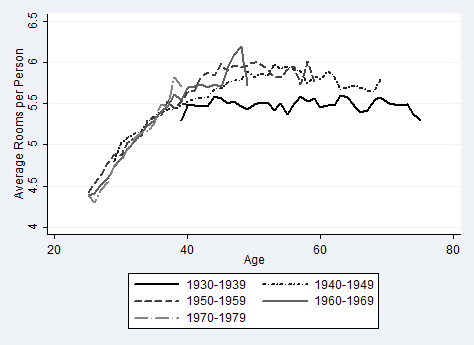
\includegraphics[width=.7\linewidth]{pictures/cohort_rooms.png}
\label{fig:cohort_rooms}
\end{figure}

\begin{figure}
\caption{Average People in Household}
\centering
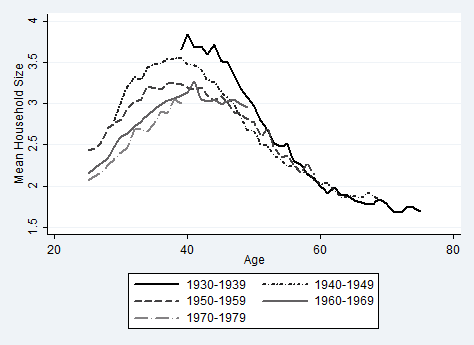
\includegraphics[width=.7\linewidth]{pictures/av_peep.png}
\label{fig:cohort_peeps}
\end{figure}



\section{Conclusion}\label{sec:conclusion}

To come.
\newpage
%\bibliographystyle{elsarticle-harv}
\bibliographystyle{ejbib}
\bibliography{library}
\newpage
\appendix
\section{Further details about the measures of income and consumption}\label{data_annex}


%\subsection{The Living Costs and Food Survey}

%The response rate in the LCFS at the start of our data period was approximately 70\% and has shown a steady decline to 52\% in the most recent year of data (REFERENCE).  These response rates are slightly lower than in the Family Resources Survey  (62\% in the recent year of data (REFERENCE)) - the survey which is used to calculate the official measures of income poverty. However, this difference comes not from large differences in the proportion refusing to participate, but from a greater number of households in the intended sample who the survey team for the LCFS fail to make contact with.


\subsection{Income}
UK government assessments of income inequality and poverty are published in a document called Households Below Average Income (hereafter HBAI), and the name is also used to describe the associated micro-dataset (the name is misleading, as the micro-data and published statistics relate to the entire income distribution). The intent is that any reasonable household survey dataset with information on household composition and sources of income could be used to derive a measure of HBAI income. The official HBAI series is based on the LCFS and its predecessors until 1993/94, and on the FRS from 1994/95;  we have generated our own equivalent series based on the LCFS from 1994/95 in order to create a consistent series based on the LCFS and its predecessors. One difference between our measure and hthe official measures after 1994/95 is that the definition of income used in the official analyses of poverty further deducts contributions by parents to any children they have who are students living outside the household, but the LCFS data does not allow us to do this. One difference between  the measure of income before and after 1994/95 us that, from 1994/95,  payments into personal pensions and maintenance payments are deducted from the measure of income.

The HBAI document sets out the precise definition of income that government statisticians are seeking to measure, and the various methods that they use for constructing the HBAI micro-data). The key factors are as follows. First, the measure of income, described as ``net household disposable income'', comprises all forms of cash income plus a very few, government-provided, near-cash benefits-in-kind, less personal taxes paid (mostly based on self-reports, although some are imputed) less some transfers to other individuals and less some forms of saving. Income is measured at the household level, and equivalised for household size and composition.  Other than some small government-provided near-cash benefits-in-kind, no allowance is made for non-cash incomes such as those from housing or unrealised capital gains. This definition of income which we hereafter call ``HBAI income'' is known in the HBAI document as income ``before housing costs [are deducted]''; an alternative measure of income, known as income ``after housing costs [are deducted]'', subtracts spending on rent, mortgage interest and water charges from BHC income. The measure differs from cash income in that includes the imputed value of free school meals for households containing children who receive them; the cash value of a free TV licence for those elderly households who are entitled to it; housing benefit that is paid direct to the landlord (the value of which is therefore not included in a household's cash income) and excludes council tax payments, payments into personal pensions, maintenance payments to those in other households and student loan repayments.

%[Mike asks: do we want this?] Table X compares the distribution of income in the LCFS and FRS for all financial years since 1994/95; in 1994/95, the two datasets gave very similar estimates of the income distribution, but in recent years, the estimate from the LCFS has been higher than that from the FRS across the distribution. The estimated Gini coefficients from both surveys are very similar, though. /footnote{The estimated Gini coefficient for the FRS incorporates an adjustment to the incomes of approximately the richest 1\% of households which has not been done for the LCFS households: see DWP (2011) for details.}]

\subsection{Imputing the consumption flow or imputed income from housing and vehicles}
As we lack data on property values, we use the rental value of the property as a measure of the consumption value of living in that property. This is (clearly) observed in the data for those households who rent their property from a private landlord. But we do not observe a rental value for owner-occupiers, and, for tenants of social landlords, we observe a rent which will typically be less than the market rent. We therefore need to estimate the rent that owner-occupiers and social tenants would pay for their property if they rented it on the private market. Our approach imputes a rent for each property based on the geographical region, the number of rooms and the local taxation bill (There were three different local taxation regimes through the period covered by our data: rates (until 1988 in England and Wales, 1989 in Scotland), the Community Charge (between the abolition of rates and 1993) and council tax (from the abolition of the Community Charge to the present). Rates and council tax both varied (positively) with the value of the property, but the Community Charge did not.).  We take households who rent an unfurnished property privately in all years of data, and split them into three groups defined by the education of the head of household (those who left school at or before age 16, those who left at age 17 or 18 and those who left at or after the age of 19); this attempts to take account partially of the fact that those at different points in the permanent income distribution might have different quality of housing that cannot be captured by the data that we observe. For each group, we estimate a median regression of the log of rent on a quadratic in local tax payments interacted with a dummy for the local tax regime (we do not allow the imputed rent of households to vary with the Community Charge), indicators for government office region, indicators for the number of rooms in the property, and indicators for financial year.  For all households, we then calculate a measure of imputed (log) housing consumption as the prediction from this median regression plus a draw from the empirical distribution of the regression residuals (the draw for a particular household is a random draw from the sample comprising the residuals for all households surveyed in the same year and with the same education level). Brzozowski and Crossley  (2010) write that ``Imputed (or predicted) rents and service flows are typically not very variable (because they are based on a small number of measured characteristics of the stocks). Including them substantially reduces the variability of the consumption bundle.'' Our procedure does not suffer from this concern, as the  (conditional-on-observables) variability in our imputed measure is, by construction, identical to that in the observed data. On the other hand, our approach implicitly assumes that this unobserved component of housing quality is uncorrelated not only with the few observables but also with income and other components of consumption.

For vehicles, we assign each household the average expenditure on vehicles by those with the same number of cars and in the same decile group of non-durable expenditure. This expenditure will be taken over the positive values of those who have purchased a car in the previous 12 months and the zero values of those who
consume but have not purchased a vehicle in the previous 12 months.

We are not able to impute credibly the consumption flow from other durables, as we do not have a comprehensive record of other durables owned. Instead, we make assume that expenditure on other durables equals consumption. An alternative (and in our view less preferred) approach is to subtract spending on other durables, without adding back an estimated consumption flow. Taking this approach, however, would make very little difference to our measure of consumption, as the ratio of durable expenditure for which we cannot credibly impute associated consumption to our measure of total consumption has a mean (median) of only 5\% (2\%).   We do not remove from consumption spending on childcare, out-of-pocket medical expenses, or education expenses. This is mostly because,  as the UK has a free-at-the-point-of-use health service, and free education for children aged  5-18, we think that any out-of-pocket spending on these items is likely to be discretionary and thus more like consumption spending than investment spending. In any case, medical and education expenses are very low in the UK (certainly compared to the US). The argument that spending on childcare should be treated as an investment is perhaps a little stronger, but the spending on childcare has not been collected in a consistent manner across the four decades; our approach of leaving it as part of consumption at least prevents us from introducing inconsistencies over time.

We note that the way in which we have added an imputed income from housing to our measures of broad income and consumption is valid only if the markets for housing and other consumer durables for which an income is imputed) are frictionless (so that we can conclude that households have equalized their marginal utility across consumption choices). /footnote{ We are very grateful to Tom Crossley for this point.}. In the case of housing, there are clear transaction costs (certainly financial and arguably psychological) to moving house. But we also note that this issue remains un-acknowledged in many papers which routinely construct a measure of income including the imputed income from housing.

\subsection{Prices indices}
[CAN WE HAVE A TABLE SHOWING RPI, THE BHC HBAI DEFLATOR, AND OUR CONSTRUCTED INDEX FOR CONSUMPTION?]

\subsection{Periodicity of income and spending}
Both the measure of spending and income in the LCFS are and measured over relatively short periods (and, because of this, conventionally reported as expressed in weekly terms). As mentioned earlier,  spending on most items is collected through diaries which cover a fortnight, but this is supplemented with estimates of the weekly spend on infrequently-purchased items, which are based on respondents' total spend over a longer period and given in response to survey questions. The concept of income in the LCFS is ``usual weekly income'': this is typically based on participants' most recent wage or salary payments (and equivalent for the other income sources), but this is then replaced with the usual wage or salary payment if the last payment was deemed by the respondent to be unusual.  So, for workers paid every month or 4 weeks, the measure of earnings is effectively usual monthly/4-weekly earnings expressed as a weekly equivalent. For workers paid weekly, the measure of earnings is usual weekly earnings.  So both income and spending are measured over much shorter periods (as well as periods that are similar to each other), than in the main US data (which measures income over the previous year, and spending over the previous quarter), but it is not the case that income and spending are collected for the same period of calendar time, as occurs, for example, in the Canadian FAMEX/SHS surveys.

\section{Supplementary results} \label{sec:annex_results}

This appendix presents variants to Tables \ref{table:multinom_incon} and \ref{table:ahc_bhc} for the earlier two decades.

%\footnotesize

\begin{table}
\caption{Income versus Consumption: 1990-1989}
\centering
\begin{tabular}{l|ccc|ccc}
\hline\hline 
	& \multicolumn{3}{c}{\textbf{BHC Bottom Decile}} &  \multicolumn{3}{c}{\textbf{AHC. Bottom Decile}} \\
	&	$r_{IC}$	&	$r_{I}$	&	$r_{C}$	&	$r_{IC}$	&	$r_{I}$	&	$r_{C}$	\\
  & se & se & se  & se & se & se \\
\hline
Left school $\leq$ 16	&	       2.446***	&	       1.371***	&	       2.828***	&	       1.369***	&	1.064	&	       1.864***	\\				
                    	&	       0.429   	&	0.072	&	0.38	&	       0.112   	&	0.044	&	0.074	\\				
Left school $>$ 19	&	       0.799   	&	       0.869*  	&	       0.654***	&	       0.822   	&	0.947	&	       0.801*  	\\				
                    	&	       0.161   	&	0.056	&	0.066	&	       0.133   	&	0.051	&	0.077	\\				
Age $<$ 30	&	       1.076   	&	       1.195** 	&	0.946	&	       1.190** 	&	       1.226***	&	       0.759*  	\\				
                    	&	       0.087   	&	0.072	&	0.09	&	       0.074   	&	0.054	&	0.088	\\				
Age 30-40	&	       1.133   	&	       1.162** 	&	       1.236*  	&	       1.021   	&	1.07	&	1.081	\\				
                    	&	       0.081   	&	0.057	&	0.126	&	       0.087   	&	0.057	&	0.138	\\				
Age 50-60	&	       0.826   	&	       0.846** 	&	1.125	&	       0.855   	&	0.922	&	1.085	\\				
                    	&	       0.103   	&	0.048	&	0.089	&	       0.121   	&	0.065	&	0.097	\\				
Age 60-70	&	       0.376***	&	       0.424***	&	       1.376** 	&	       0.149***	&	       0.368***	&	1.146	\\				
                    	&	       0.049   	&	0.03	&	0.145	&	       0.019   	&	0.032	&	0.135	\\				
Age $\geq$ 70	&	       0.424***	&	       0.233***	&	       2.399***	&	       0.233***	&	       0.226***	&	       2.183***	\\				
                    	&	       0.053   	&	0.025	&	0.286	&	       0.036   	&	0.024	&	0.294	\\				
Unemployed	&	       7.997***	&	       4.224***	&	       2.517***	&	      10.829***	&	       4.365***	&	       3.137***	\\				
	&	       0.918   	&	0.254	&	0.094	&	       1.296   	&	0.291	&	0.14	\\				
Constant            	&	       0.014***	&	       0.028***	&	       0.026***	&	       0.014***	&	       0.040***	&	0.179	\\				
                    	&	       0.003   	&	0.002	&	0.004	&	       0.002   	&	0.004	&	       2.801***	\\
\hline\hline
\multicolumn{7}{l}{Significantly different from zero at the 5\% ($\star\star$) and 1\% level ($\star\star\star$).} \\
\multicolumn{7}{l}{Omitted variables: Left school between 17-18 years old, household head aged between} \\
\multicolumn{7}{l}{40 and 50 years, employed. Controls for household composition.}
\end{tabular}
\end{table}

\begin{table}
\caption{Income versus Consumption: 1980-1989}
\centering
\begin{tabular}{l|ccc|ccc}
\hline\hline 
	& \multicolumn{3}{c}{\textbf{BHC Bottom Decile}} &  \multicolumn{3}{c}{\textbf{AHC. Bottom Decile}} \\
	&	$r_{IC}$	&	$r_{I}$	&	$r_{C}$	&	$r_{IC}$	&	$r_{I}$	&	$r_{C}$	\\
  & se & se & se  & se & se & se \\
\hline
Left school $\leq$ 16	&	       2.171***	&	       1.233** 	&	       2.025***	&	       1.603***	&	       1.137*  	&	       2.123***	\\				
                    	&	       0.270   	&	0.079	&	0.192	&	       0.199   	&	0.06	&	0.144	\\				
Left school $>$ 19	&	       0.615*  	&	       0.815*  	&	0.681	&	       0.597** 	&	0.919	&	0.835	\\				
                    	&	       0.140   	&	0.071	&	0.149	&	       0.116   	&	0.046	&	0.107	\\				
Age $<$ 30	&	       0.918   	&	       1.294***	&	0.965	&	       0.980   	&	       1.346***	&	1.163	\\				
                    	&	       0.081   	&	0.078	&	0.081	&	       0.131   	&	0.078	&	0.124	\\				
Age 30-40	&	       1.070   	&	1.026	&	1.188	&	       0.873   	&	0.98	&	1.143	\\				
                    	&	       0.095   	&	0.075	&	0.108	&	       0.101   	&	0.065	&	0.097	\\				
Age 50-60	&	       0.757*  	&	0.892	&	0.873	&	       0.809   	&	       0.830** 	&	0.825	\\				
                    	&	       0.087   	&	0.073	&	0.169	&	       0.089   	&	0.053	&	0.146	\\				
Age 60-70	&	       0.404***	&	       0.536***	&	       1.488** 	&	       0.236***	&	       0.372***	&	       1.459** 	\\				
                    	&	       0.034   	&	0.073	&	0.188	&	       0.039   	&	0.044	&	0.174	\\				
Age $\geq$ 70	&	       0.639***	&	       0.370***	&	       3.077***	&	       0.369***	&	       0.254***	&	       3.107***	\\				
                    	&	       0.064   	&	0.041	&	0.297	&	       0.056   	&	0.028	&	0.297	\\				
Unemployed	&	      13.615***	&	       6.035***	&	       2.510***	&	      18.302***	&	       7.111***	&	       3.140***	\\				
                    	&	       0.901   	&	0.858	&	0.121	&	       1.212   	&	0.828	&	0.104	\\				
Constant            	&	       0.004***	&	       0.015***	&	       0.013***	&	       0.004***	&	       0.018***	&	       0.011***	\\				
                    	&	       0.001   	&	0.002	&	0.002	&	       0.001   	&	0.003	&	0.002	\\
\hline\hline
\multicolumn{7}{l}{Significantly different from zero at the 5\% ($\star\star$) and 1\% level ($\star\star\star$).} \\
\multicolumn{7}{l}{Omitted variables: Left school between 17-18 years old, household head aged between} \\
\multicolumn{7}{l}{40 and 50 years, employed. Controls for household composition.}
\end{tabular}
\end{table}

\begin{table}
\caption{AHC versus BHC: 1990-1999}
\centering
\begin{tabular}{l|ccc|ccc}
\hline\hline 
	& \multicolumn{3}{c}{\textbf{Income Bottom Decile}} &  \multicolumn{3}{c}{\textbf{Cons. Bottom Decile}} \\
	&	$r_{AB}$	&	$r_{A}$	&	$r_{B}$	&	$r_{AB}$	&	$r_{A}$	&	$r_{B}$	\\
  & se & se & se  & se & se & se \\
\hline
Left school $\leq$ 16	&	       1.226***	&	       2.486***	&	       0.700***	&	       2.390***	&	       2.891***	&	1.054	\\
                    	&	       0.055   	&	0.216	&	0.072	&	       0.265   	&	0.363	&	0.083	\\
Left school $>$ 19	&	       0.860** 	&	       0.526***	&	1.041	&	       0.709*  	&	       0.497***	&	0.877	\\
                    	&	       0.045   	&	0.066	&	0.134	&	       0.102   	&	0.079	&	0.153	\\
Age $<$ 30	&	       1.486***	&	1.096	&	       1.435***	&	       1.181*  	&	1.207	&	1.073	\\
                    	&	       0.089   	&	0.106	&	0.133	&	       0.098   	&	0.122	&	0.099	\\
Age 30-40	&	       1.294***	&	       1.526***	&	1.023	&	       1.406***	&	       1.651***	&	1.104	\\
                    	&	       0.063   	&	0.128	&	0.091	&	       0.126   	&	0.108	&	0.172	\\
Age 50-60	&	       0.725***	&	       0.368***	&	0.979	&	       0.766*  	&	       0.621***	&	       1.320** 	\\
                    	&	       0.035   	&	0.054	&	0.115	&	       0.079   	&	0.039	&	0.118	\\
Age 60-70	&	       0.274***	&	       0.270***	&	       0.354***	&	       0.583***	&	       0.493***	&	1.103	\\
                    	&	       0.016   	&	0.043	&	0.047	&	       0.073   	&	0.036	&	0.155	\\
Age $\geq$ 70	&	       0.159***	&	       0.259***	&	       0.364***	&	       1.155   	&	       0.658***	&	       2.205***	\\
                    	&	       0.016   	&	0.041	&	0.046	&	       0.161   	&	0.043	&	0.295	\\
Unemployed	&	       5.249***	&	       6.063***	&	       7.492***	&	       4.816***	&	       3.289***	&	       4.494***	\\
	&	       0.336   	&	0.51	&	0.406	&	       0.289   	&	0.255	&	0.366	\\
Constant            	&	       0.075***	&	       0.024***	&	       0.051***	&	       0.053***	&	       0.029***	&	       0.044***	\\
                    	&	       0.006   	&	0.003	&	0.008	&	       0.008   	&	0.003	&	0.007	\\
\hline\hline
\multicolumn{7}{l}{Significantly different from zero at the 5\% ($\star\star$) and 1\% level ($\star\star\star$).} \\
\multicolumn{7}{l}{Omitted variables: Left school between 17-18 years old, household head aged between} \\
\multicolumn{7}{l}{40 and 50 years, employed. Controls for household composition.} 
\end{tabular}
\end{table}

\begin{table}
\caption{AHC versus BHC: 1980-1989}
\centering
\begin{tabular}{l|ccc|ccc}
\hline\hline 
	& \multicolumn{3}{c}{\textbf{Income Bottom Decile}} &  \multicolumn{3}{c}{\textbf{Cons. Bottom Decile}} \\
	&	$r_{AB}$	&	$r_{A}$	&	$r_{B}$	&	$r_{AB}$	&	$r_{A}$	&	$r_{B}$	\\
  & se & se & se  & se & se & se \\
\hline
Left school $\leq$ 16	&	       1.198** 	&	       1.985***	&	0.874	&	       2.237***	&	       2.019***	&	       1.230*  	\\
                    	&	       0.077   	&	0.165	&	0.096	&	       0.184   	&	0.257	&	0.112	\\
Left school $>$ 19	&	       0.822** 	&	       0.582*  	&	1.1	&	       0.706   	&	0.677	&	1.078	\\
                    	&	       0.055   	&	0.13	&	0.158	&	       0.163   	&	0.185	&	0.21	\\
Age $<$ 30	&	       1.624***	&	       1.206*  	&	       1.800***	&	       1.289** 	&	1.047	&	       1.376*  	\\
                    	&	       0.102   	&	0.107	&	0.188	&	       0.124   	&	0.096	&	0.216	\\
Age 30-40	&	       1.354***	&	       1.618***	&	1.204	&	       1.427***	&	       1.603***	&	1.022	\\
                    	&	       0.089   	&	0.139	&	0.127	&	       0.123   	&	0.092	&	0.139	\\
Age 50-60	&	       0.687***	&	       0.495***	&	1.012	&	       0.754*  	&	       0.499***	&	1.159	\\
                    	&	       0.032   	&	0.043	&	0.073	&	       0.102   	&	0.052	&	0.113	\\
Age 60-70	&	       0.346***	&	       0.455***	&	       0.584** 	&	       0.928   	&	       0.517***	&	       1.505***	\\
                    	&	       0.040   	&	0.047	&	0.109	&	       0.088   	&	0.042	&	0.134	\\
Age $\geq$ 70	&	       0.265***	&	       0.601***	&	       0.650*  	&	       2.193***	&	       0.793***	&	       2.967***	\\
                    	&	       0.037   	&	0.07	&	0.111	&	       0.199   	&	0.041	&	0.275	\\
Unemployed	&	       8.440***	&	       7.189***	&	      12.197***	&	       4.969***	&	       4.038***	&	       5.608***	\\
	&	       0.903   	&	0.451	&	0.738	&	       0.210   	&	0.277	&	0.396	\\
Constant            	&	       0.051***	&	       0.014***	&	       0.024***	&	       0.028***	&	       0.020***	&	       0.018***	\\
                    	&	       0.006   	&	0.002	&	0.005	&	       0.003   	&	0.002	&	0.003	\\
\hline\hline
\multicolumn{7}{l}{Significantly different from zero at the 5\% ($\star\star$) and 1\% level ($\star\star\star$).} \\
\multicolumn{7}{l}{Omitted variables: Left school between 17-18 years old, household head aged between} \\
\multicolumn{7}{l}{40 and 50 years, employed. Controls for household composition.} \end{tabular}
\end{table}


%\section{Old text on housing} \label{sec:annex_housing}

[OLD TEXT FROM SECTION ON HOUSING/COHORTS]

The results discussed above show that adding the imputed resources from housing reduces the slope of the age profile of poverty.  Figure \ref{fig:pov_age} probes this result more, by showing the age profile of being in the bottom decile group of [Mike asks Abi: is this income or consumption? Could we have both?] for different birth cohorts with and without the imputed resources from housing. The key points are as follows. First, however measured, the age profile of poverty is becoming less steep for successive birth cohorts. [Mike asks Abi: some of the numbers in the figures are very low - just a $2\%$ chance of being in the bottom decile? Also, I am concerned that some of these look q different from Figures 40-42 of the Brewer-O'Dea WP.] This is in line with findings in [XXXX] that old age is no longer a good predictor for being in the poorest group (although they confound age and cohort). More importantly for our analysis, though, is that the age profile of being in the bottom decile group of income/consumption [which?] including imputed resources from housing is becoming increasingly less steep over time than the age profile of being in the bottom decile group of income/consumption without imputed resources from housing. Indeed, for the 1950s cohort, the age profile  of being in the bottom decile group of income/consumption with imputed resources from housing is broadly flat (at least after the late 30s), whereas it remains upward sloping (at least above age 40) when resources are measured without those from housing.

[Mike asks ABi and COrmac: I still find myself wanting to show how the cohort-profile of poverty in a given year as changed over time (as we did in the WP). Can we? please?]

Clearly, many of these results are due to the age- and cohort- patterns in the ownership of housing, and the value of that implicit consumption or income that home-owners enjoy. Panel (a) of Figure \ref{fig:room_age_tenure} shows the fraction of individuals/households [which?] who live in owner-occupied housing by age and cohort. The life-cycle pattern is unsurprising, with home-ownership rising steeply between mid 20s to the mid 40s, and more slowly thereafter. But the figure also reveals the striking cohort patterns: for a given age, home-ownership is the most likely for the 1940s and 1950s cohorts, and less likely for all others.  [Mike asks Abi: are these raw data? Smoothed? from an APC analysis? we probably need to give detail on how these were created or smoothed etc].

Panel (b) of Figure \ref{fig:room_age_tenure} does a similar analysis for the number of rooms [Mike asks Abi: precise definition?] occupied by households who own their own house [Mike asks Abi: is this right? i.e is it conditional on owning a property?]. [Mike asks Abi and Cormac: I am not sure what it shows. And we discussed that there seems to be a time effect, in that all cohorts see a fall in number rooms in 2000. We noted this when we met, and I have an email (sent by me 13/03/2015) saying that Cormac was going to look at this, but I don't have a record of the answer].


\begin{figure}
\caption{Risk of Poverty, by Age and Cohort }
\centering
\begin{tabular}{c c}
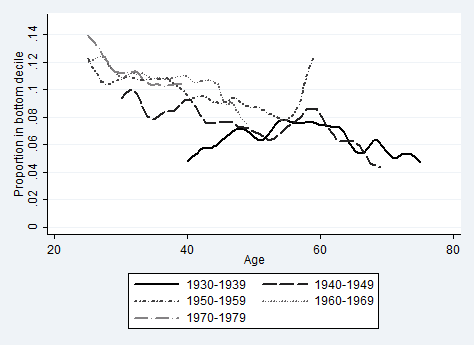
\includegraphics[width=.5\linewidth]{pictures/cohortagerisksmooth_bhc_inc.png} &
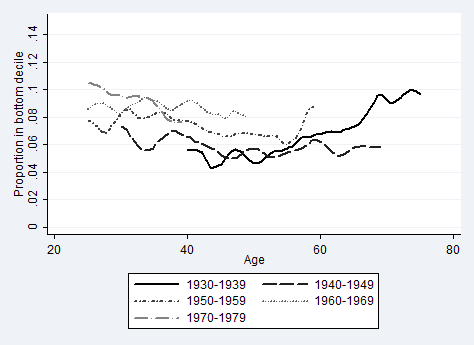
\includegraphics[width=.5\linewidth]{pictures/cohortagerisksmooth_bhc_con.png} \\
(a) Income inc. Housing & (b) Consumption inc. Housing \\
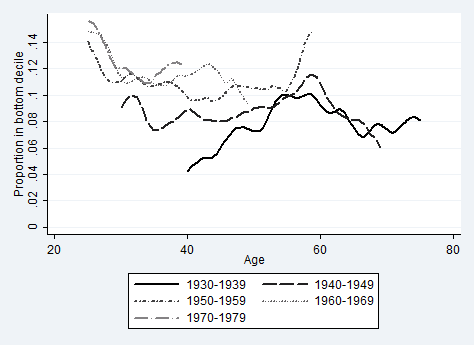
\includegraphics[width=.5\linewidth]{pictures/cohortagerisksmooth_ahc_inc.png} &
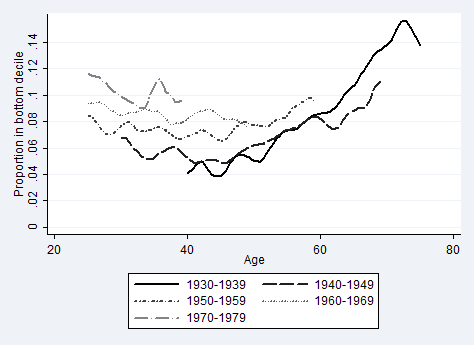
\includegraphics[width=.5\linewidth]{pictures/cohortagerisksmooth_ahc_con.png} \\
(c) Income ex. Housing & (d) Consumption ex. Housing \\
\end{tabular}
\label{fig:povage_cohort}
\end{figure}

\begin{figure}
\caption{Risk of Poverty, by Age and Cohort }
\centering
\begin{tabular}{c c}
Income & Consumption\\
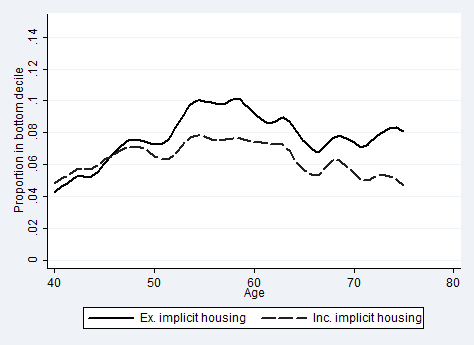
\includegraphics[width=.5\linewidth]{pictures/cohort2_agerisksmooth_inc.png} &
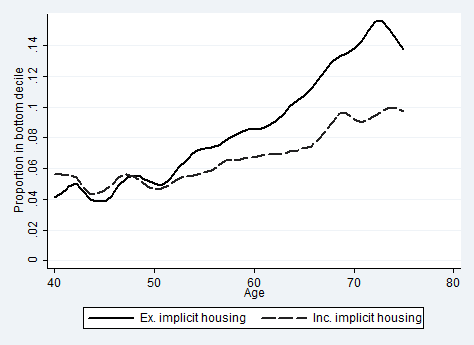
\includegraphics[width=.5\linewidth]{pictures/cohort2_agerisksmooth_con.png} \\
(a) 1930s Cohort & (b) 1930s Cohort \\
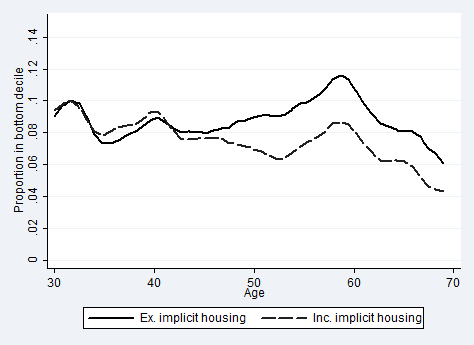
\includegraphics[width=.5\linewidth]{pictures/cohort3_agerisksmooth_inc.png} &
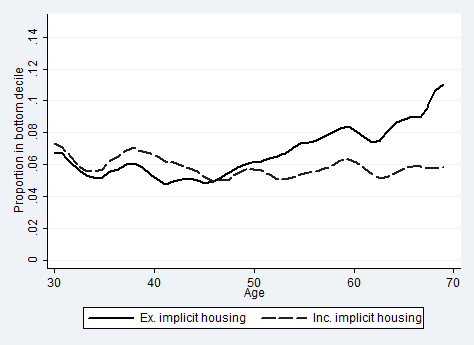
\includegraphics[width=.5\linewidth]{pictures/cohort3_agerisksmooth_con.png} \\
(c) 1940s Cohort & (d) 1940s Cohort \\
\end{tabular}
\label{fig:povage_cohort_restrict}
\end{figure}


\begin{figure}
\caption{Average Rooms Occupied per Person}
\centering
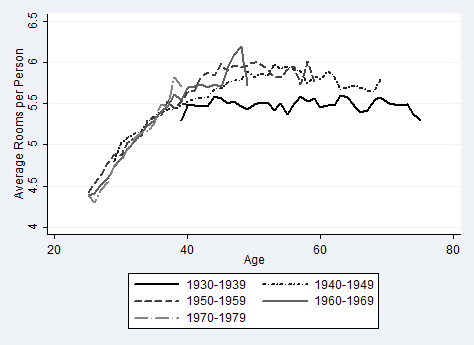
\includegraphics[width=.7\linewidth]{pictures/cohort_rooms.png}
\label{fig:cohort_rooms}
\end{figure}

\begin{figure}
\caption{Average People in Household}
\centering
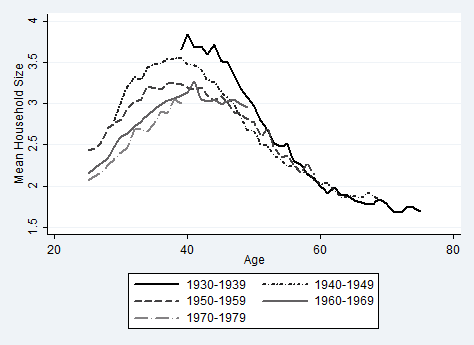
\includegraphics[width=.7\linewidth]{pictures/av_peep.png}
\label{fig:cohort_peeps}
\end{figure}


\begin{figure}
\caption{Average Rooms per Person, 1979-2000}
\centering
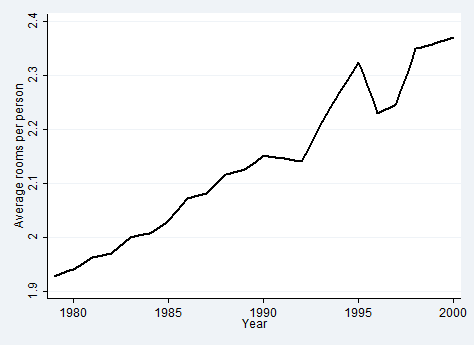
\includegraphics[width=0.7\linewidth]{pictures/rooms_pp.png}
\label{fig:room_time}
\end{figure}






\end{document}
%
%todo
%Literature review is not great, and needs amending as suggested in text. Also look at literature on developing countries
%References and bibliography
%chapter 3: refer to BEOD
%all: rewrite AHC and BHC
%Ask Abi how did bootstrap
%why leave out the recession? 
%discuss statistical significance in section 4
% notes and sources to all figures
% some figures look different from the original WP